%\sectskip
\section{Verifying the {\cCTOS} Kernel}
\label{sec:con:base}
%\asectskip

\ignore{
\begin{figure}
\begin{minipage}{.22\textwidth}
\lstinputlisting [language = C] {source_code/lock_producer.c}
\end{minipage}\hfill
\begin{minipage}{.22\textwidth}
\lstinputlisting [language = C] {source_code/lock_consumer.c}
\end{minipage}
\ifTR{}{\vspace*{-5pt}}
\caption{Lock-based producer-consumer implementation}
\label{fig:exp:lock}
\end{figure}
}


\begin{comment}
\begin{figure*}
\begin{center}
\begin{scriptsize}
\begin{tabular}{ |l|l||l|p{4.5cm}| }
  \hline
  \multicolumn{2}{|c||}{\textbf{Memory Management}} 
  & \multicolumn{2}{|c|}{\textbf{Thread and Process Management}} \\
  \hline
  \hline    
  \multicolumn{2}{|l||}{\textbf{abstract state}} 
  & \multicolumn{2}{|l|}{\textbf{abstract state}}\\
  \hline
  \verb"AT" & physical page allocation table
  & \verb"kctxp" & kernel context (\verb"kctx") pool\\
  \hline 
  \verb"PFInfo" & save the address and \verb"PC" that page fault occurs
  & \verb"Ltdqp" & low abstract thread queue pool\\
  \hline
  \verb"ptp" & page table (\verb"pt") pool 
  
  & \verb"Htdqp"& high abstract thread queue (\verb"Htdq") pool\\ 
  \hline
   \verb"ipt"& whether \verb"pt"'s invariant  should hold or not
  
  & \verb"uctxp" & user context pool\\
  \hline
\verb"PT" & index of the current \verb"pt"
  & \verb"chanp" & channel pool\\
  \hline
  \verb"pbit" & bit map for free \verb"pt" indexes
  & \verb"Htcbp"& high abstract TCB pool \\
  \hline
  \multicolumn{2}{|l||}{\textbf{primitive}} 
  & \multicolumn{2}{|l|}{\textbf{primitive}}\\
  \hline	
  \verb"setcr3" & set the starting address of the \verb"pt"
  & \verb"kctx_new" & allocate the first free \verb"pt" and \verb"kctx"\\
  \hline
  \verb"meminit" & initialize the allocation table
  & \verb"Henqueue" & append a thread to the \verb"Htdq"\\
  \hline
  \verb"palloc" & allocate a page 
  & \verb"thread_kill" & kill and free a thread\\
  \hline
  \verb"pt_insrt" & insert a page map into a given \verb"pt" 
  & \verb"thread_sleep" & sleep, schedule to the 1st ready thread\\
  \hline
  \verb"pt_resv" & allocate a page for a given linear addr 
  & \verb"kctx_switch" & switch \verb"kctx" between threads\\
  \hline 
  \verb"PTInit" & init kernel's \verb"pt" and enable paging 
  & \multirow{2}{*}{\texttt{resv\_chan}} & 
  receive msg from the channel, wake\\
  \cline{1-2}
  \verb"pt_new" & allocate the first free \verb"pt" & & up the first sleeping thread
    \\	  
  \hline
  \hline
  \multicolumn{2}{|c||}{\textbf{Virtualization}}
  &\multicolumn{2}{|c|}{\textbf{Trap Handler}} \\
  \hline
  \hline    
  \multicolumn{2}{|l||}{\textbf{abstract state}} 
  & \multicolumn{2}{|l|}{\textbf{primitive}} \\
  \hline
  \verb"npt" & nested page table for guest
  & \verb"trap_arg" & get arguments of system calls\\
  \hline
  \verb"hctx"& host context
  & \verb"hpagefault" & page fault handler\\ 
  \hline
  \verb"vmcb" & virtual machine (\verb"VM") control control block
  & \verb"sys_yield" & system calls for yielding\\
  \hline
  \verb"xvmst" & registers not saved in \verb"vmcb" 
  & \verb"sys_wait_chan" & system calls to sleep on a channel\\
  \hline
  \multicolumn{2}{|l||}{\textbf{primitive}} 
  & \verb"sys_run_vm" & system calls to run \verb"VM"\\
  \hline	
  \verb"npt_insrt" & insert into the nested page table
  & \verb"sys_proc_create" & system calls to create a process\\
  \hline
  \verb"switch2guest" &  switch to guest mode 
  & \verb"sys_getexitinfo" 
  & get the information about \verb"VM" exit\\
  \hline
  \verb"set_vmcb" & set value in virtual machine control block
  & \verb"sys_injectevent" & inject interrupt and exception to \verb"VM"\\
  \hline 
  \verb"run_vm" & save host context, restore \verb"vmcb", start \verb"VM" 
  & \verb"kernel_init" & initialization function of the kernel\\  
  \hline  

\end{tabular}
\end{scriptsize}
\caption{Key abstract states and primitives for \mCTOSbase{} and \mCTOShyper{}}
\label{table:layers}
\end{center}
%\vspace*{-14pt}
\end{figure*}
\end{comment}

\begin{comment}
\begin{figure}
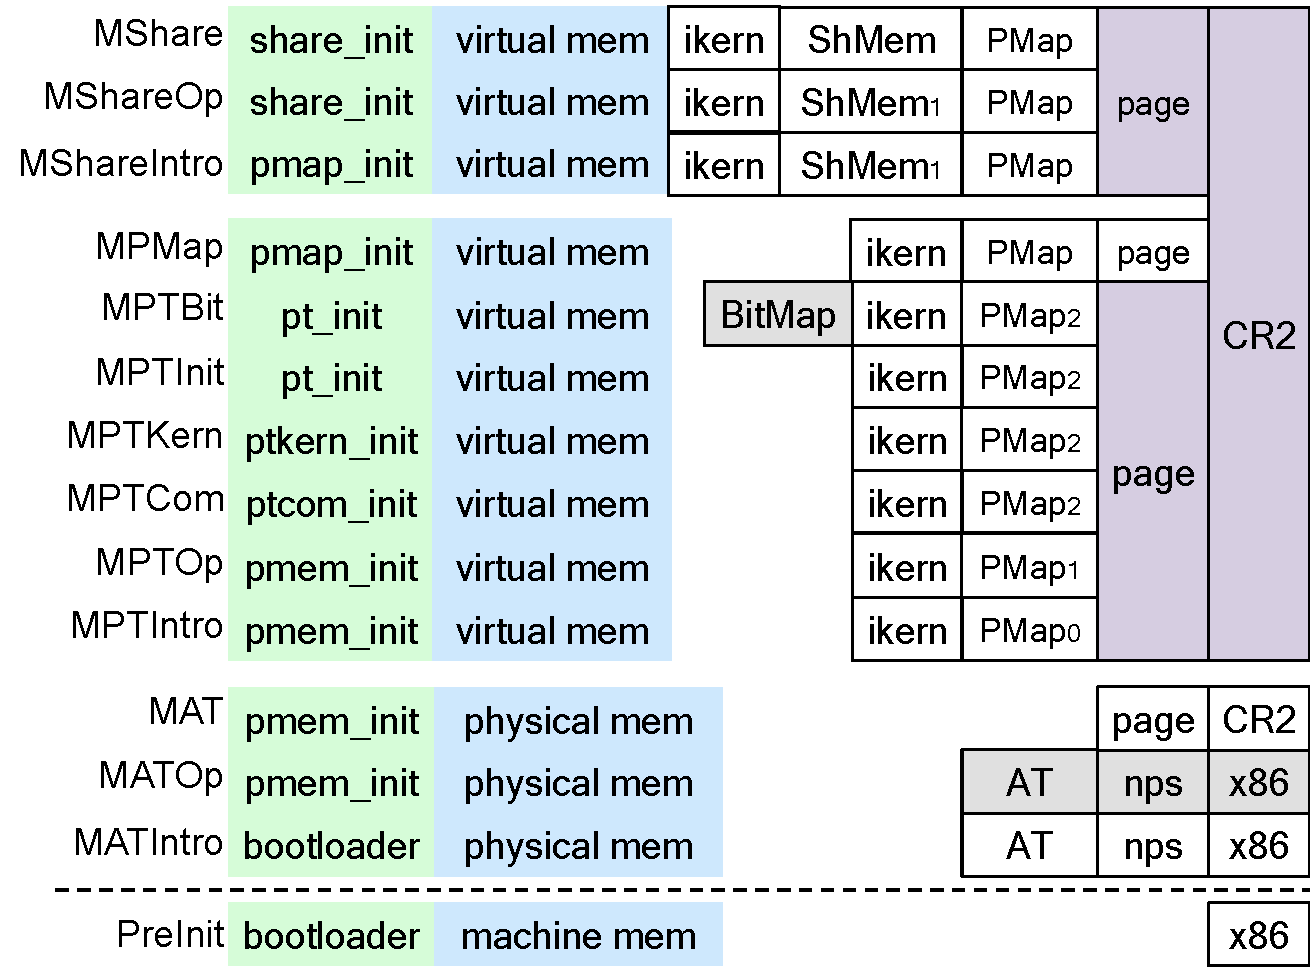
\includegraphics[scale=0.38]{figs/memory_management_layer}	
\caption{Layers of PreInit and memory management}
\label{fig:base:mm:layers}
\vspace*{-14pt}
\end{figure}

\begin{figure}
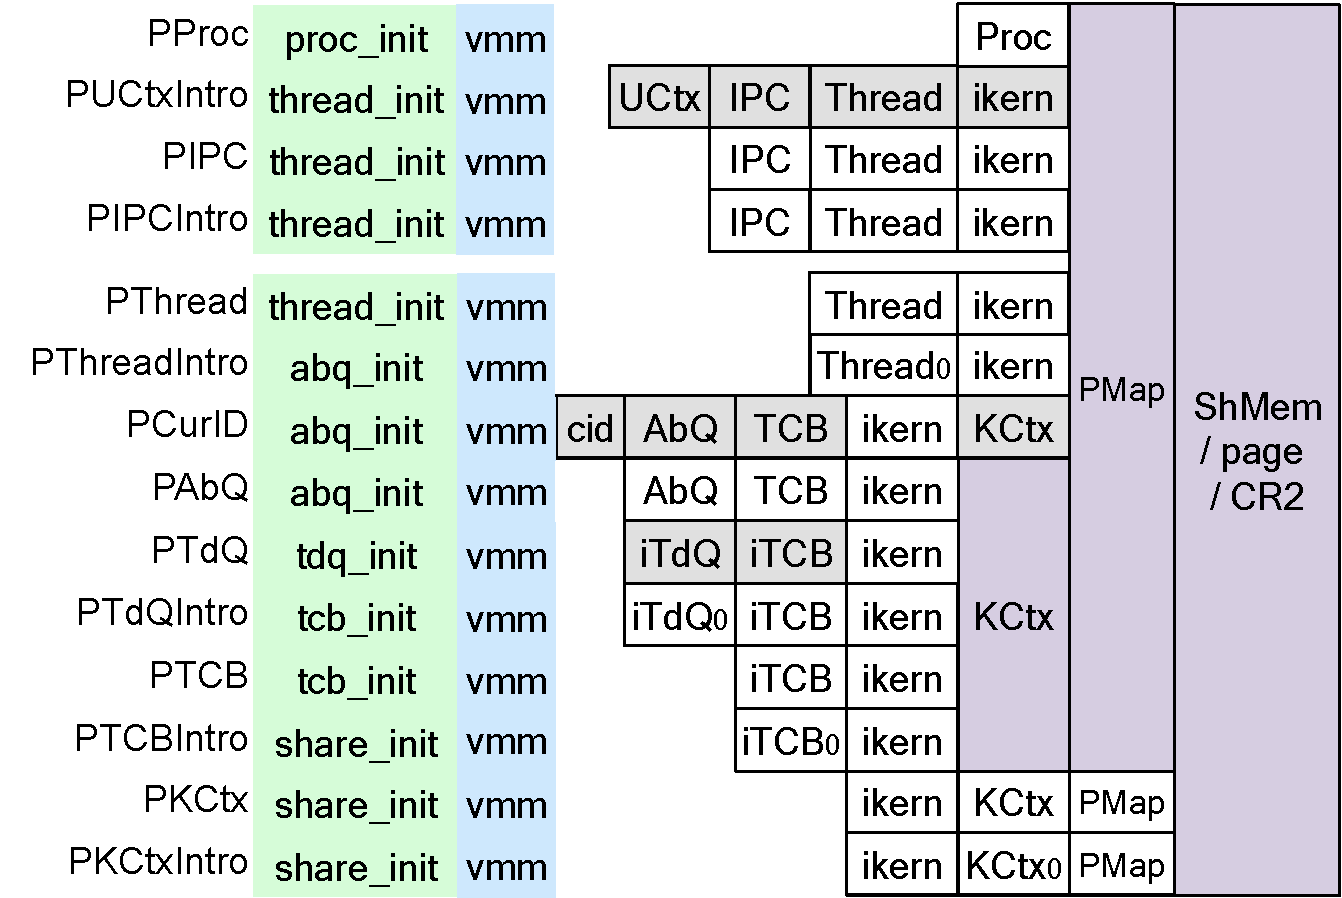
\includegraphics[scale=0.37]{figs/process_management_layer}	
\caption{Layers of process management}
\label{fig:base:pm:layers}
\vspace*{-14pt}
\end{figure}

\begin{figure}
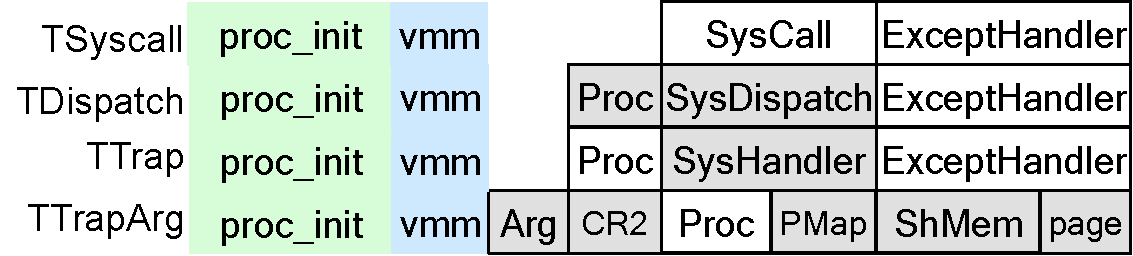
\includegraphics[scale=0.37]{figs/trap_management_layer}	
\caption{Layers of trap management}
\label{fig:base:tm:layers}
\vspace*{-14pt}
\end{figure}
\end{comment}

\ignore{
\begin{figure}
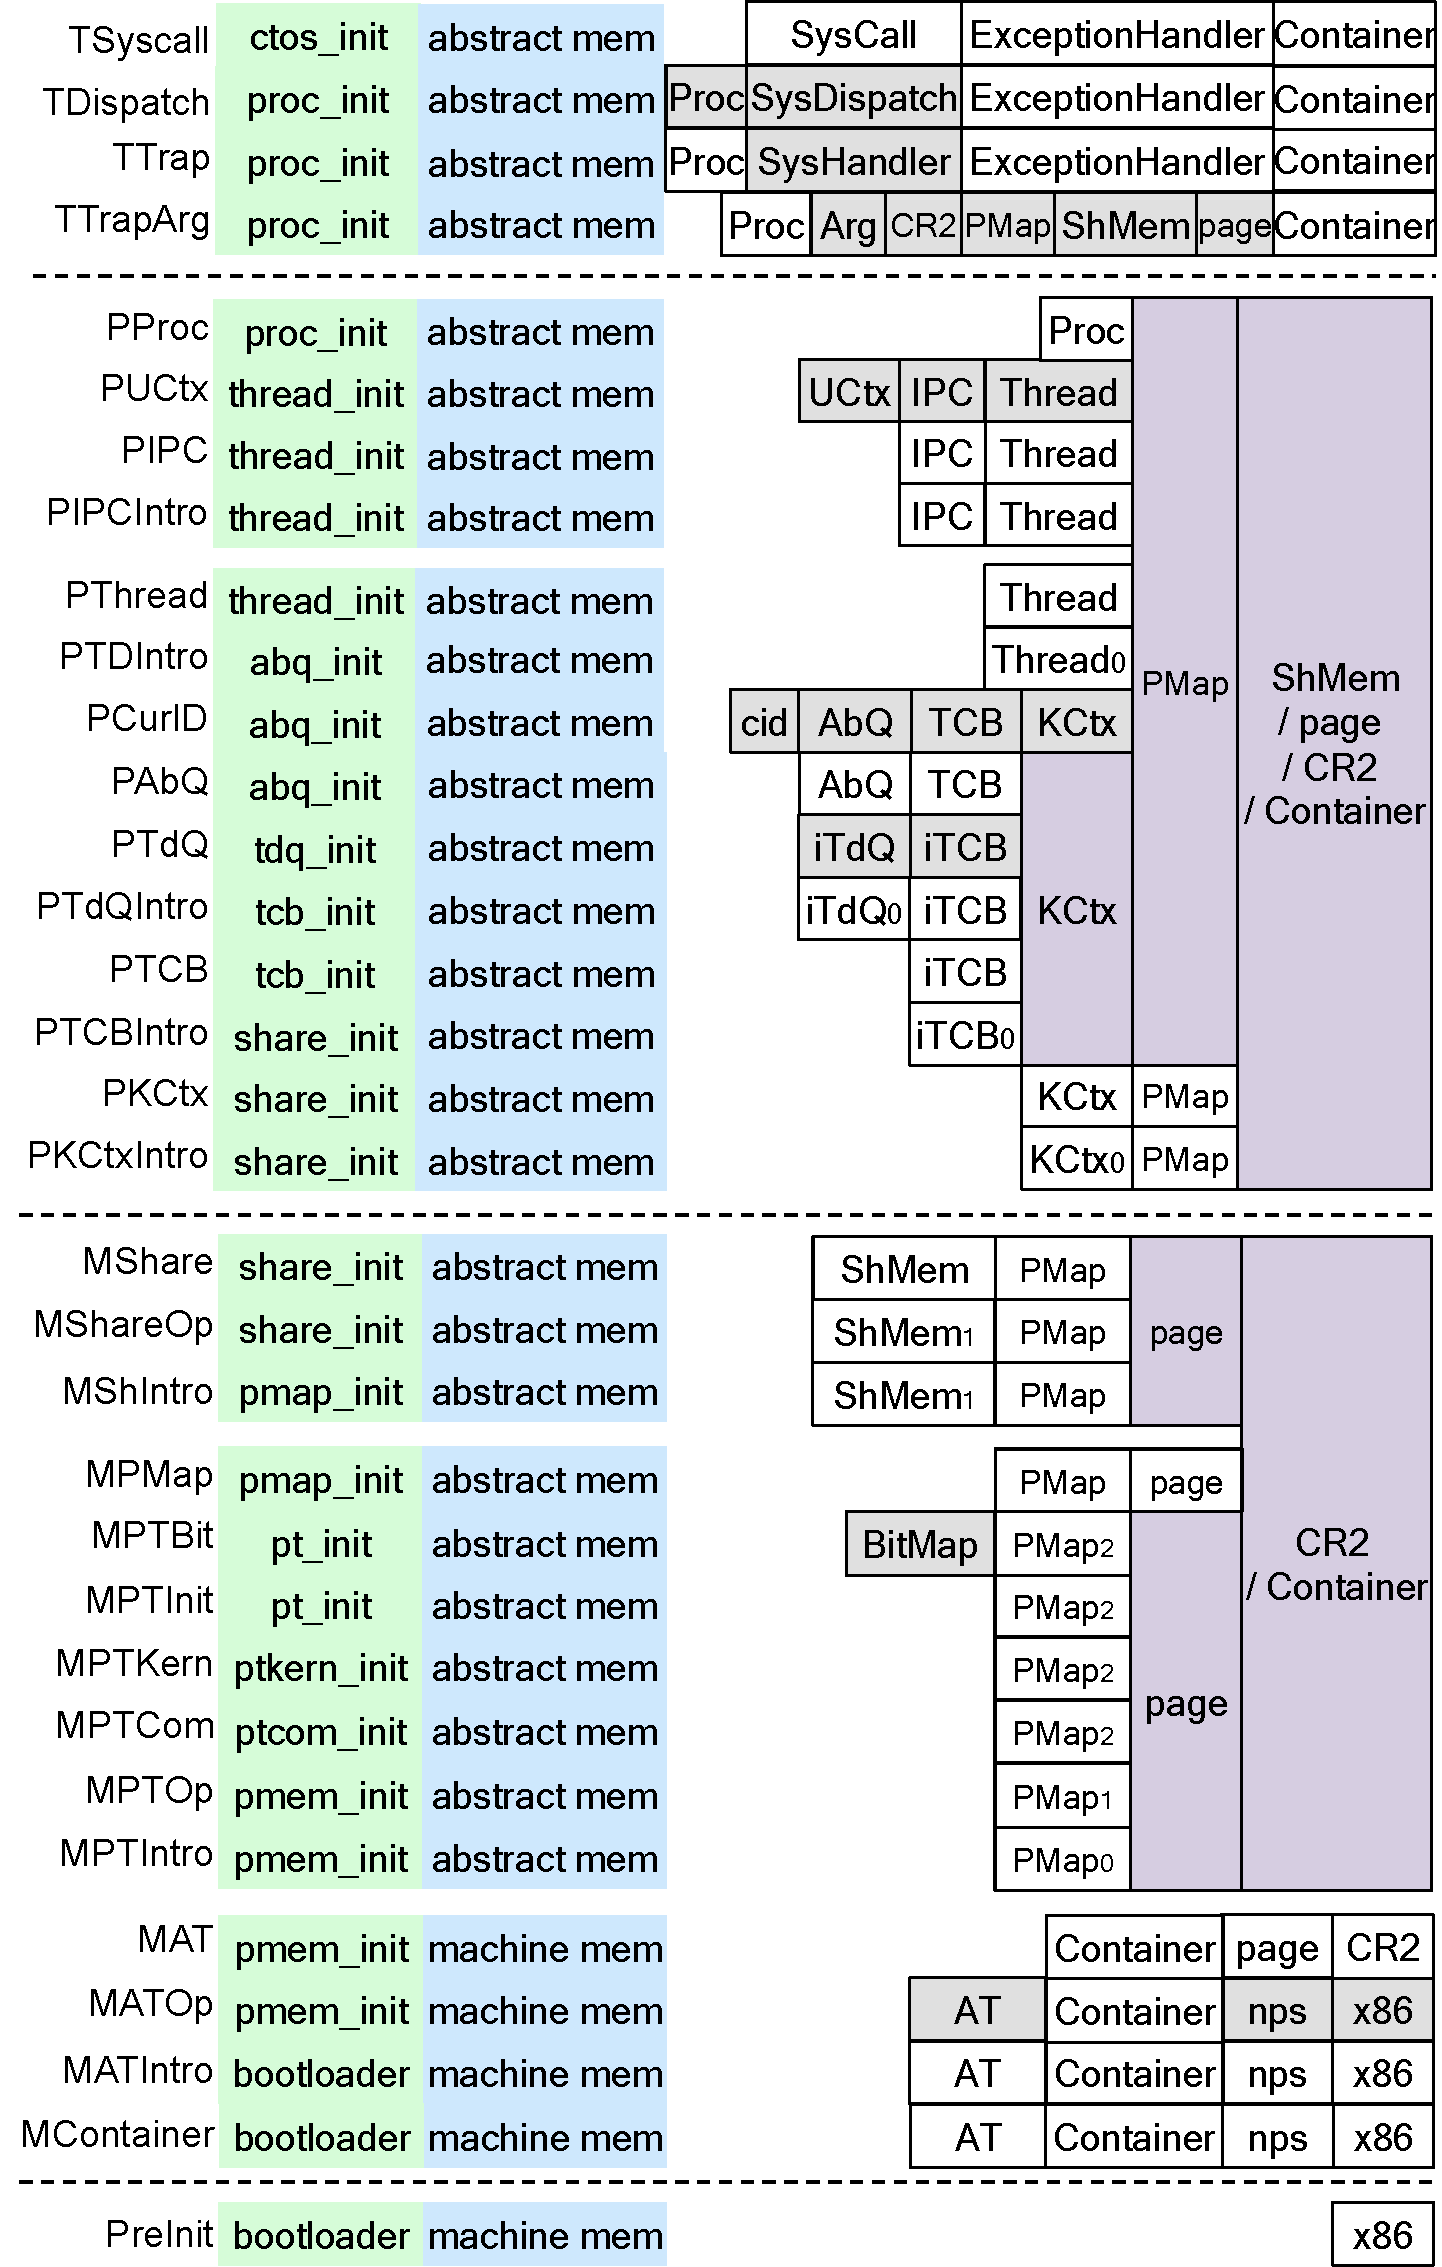
\includegraphics[scale=0.34]{figs/mctos_layer}	
\caption{Layers of \mCTOSbase{}}
\label{fig:base:ctos:layers}
\vspace*{-14pt}
\end{figure}
}

In this section, we present the main components of the certified {\cCTOS} kernel. 
The pre-initialization module is the bottom layer $L_\boot$
that connects to the
 \emph{CPU-local machine model} $\pmach{loc}$, instantiated with a 
 particular \emph{active CPU} (\cf Section~\ref{sec:con:lasm}).
The trap handler contains the top layer that provides system call interfaces
and serves as a specification of the whole kernel,
instantiated with a particular active thread
running on that active CPU.
Our main theorem states that any global properties proved at the topmost
abstraction layer can be transferred down to the lowest hardware machine.
In this section, we show
how to verify 
the concurrent objects in \cCTOS{}
(\ie, spinlocks, shared queues protected by spinlocks,
thread scheduler, and a queuing lock)
and other extensions to the sequential
kernel \mCTOS{}
using concurrent abstraction layers.
All layers are built upon the single-core machine $\LAsm{(L(c,\oracle))}$.

\ignore{
\paragraph{Pre-initialization module}
\label{sec:base:preinit}
only contains the bottommost layer
\code{PreInit}. It axiomatizes the x86 hardware behaviors of a particular active CPU.
These behaviors include page table walk upon memory load when paging is turned on, 
saving and restoring the trap frame in the case of interrupts and exceptions (\eg, page fault), 
and the data exchange between devices and memory.
\ignore{The abstract state of the \code{PreInit} layer consists of control registers, FLAGS registers,
registers of devices, an E820 memory map \code{MM} (set up by the bootloader),
and a CPU-mode flag (either kernel or user mode).
\ignore{Its primitives consist of
getter-setter functions for control registers and \code{MM},
and a function models the transition between user and kernel mode.}
}

As shown in Fig.~\ref{fig:spec:memmodel}(a),
the hardware memory management unit (MMU) is modeled 
in a way that mirrors the paging hardware.
When paging is enabled (as indicated by \code{CR0}),
memory accesses made by both the kernel and the user programs
are translated using the page map pointed to by \code{CR3}.
When a page fault occurs,
the fault information is stored in \code{CR2},
the CPU mode is switched from user mode to kernel mode,
and the page fault handler is triggered.
}
\ignore{
Some privileged
memory regions (\eg, allocation table) and 
instructions (\eg, modifying control registers)
are only available in kernel mode.}
\ignore{
\code{CR0} selects the memory protection mode,
\code{CR2} stores the Page Fault Linear Address (PFLA)
as well as the address of the instruction that caused the page fault, and
\code{CR3} stores the starting point of the page map.
}
\ignore{
The switch function models the change of the \code{ikern} flag
and the remaining tasks involved with trap handling,
such as saving and restoring user and kernel contexts,
and dispatch over the trap type,
are verified at the assembly level.
}


\subsection{Ticket lock module}
\label{sec:base:lock}

\ignore{
\subsection{Layer interfaces}
\label{sec:prog:layer}
We enable abstraction in our framework by
instrumenting concrete memory states with abstract
state and logical log components. 
Both abstract state and logical logs can be manipulated using
primitives, which are made available through CompCert’s external
function mechanism.

\paragraph{Machine state}
for a single core $c$ 
 is defined as $\state:=(\regs, m, a, l)$,
which consists of the CPU-local state $\regs$,
shared memory state $m$, 
abstract state $a$, and a global log $l$. 
%The assembly language
%contains an extra register set component $regset$.

\textbf{Local state} $\regs$ consists of the CPU-local memory state,
which is invisible to other CPUs,
and the language-dependent local components.
\ignore{The local memory is a sequence of CompCert memory blocks\ronghui{reference here, Tahina} \tahina{Do we really need to say here that we are using the CompCert memory model?},
which can be addressed by the block identifier and the offset within the block. This part of the memory is  private to a single CPU,
and are invisible to other CPUs.
The rest of the local components are language dependent.}
For instance, a C-like language includes 
a local/temporary environment and a continuation,
while an assembly language contains a register set.

\textbf{Shared memory state}  $m$ is \ignore{also  a sequence of
memory blocks, which are }shared among all CPUs.
Each shared memory location is associated
with a valid bit, which can only be manipulated by
atomic shared operations (\ie, $\pull$ and $\push$). The $\pull$ operation
sets an invalid bit to valid, only after which can shared memory accesses
be performed. The $\push$ operation invalidates the bit
and records the shared memory updates to the logical log.
If a program tries to pull a shared memory location that is already valid,
there is a \emph{data race} and the machine gets \emph{stuck}.
One goal of concurrent program verification is to show
that a program is data-race free.
In our setting, we accomplish this by showing that the program does not 
get stuck.

\textbf{Abstract state} $a$ is not just a ghost state for reasoning.
Instead, it is abstracted from a concrete in-memory data structure,
and it can influence the outcome of program executions.
It is used to hide implementation details and to lift reasoning
to a purely logical level. Access to an abstract state can only
be performed via explicit calls to primitives.
\ignore{
\newman{Duplicated}
, which are implemented
as Clight’s external function calls. This minimizes the impact on the
semantics of C and assembly languages.
}

\textbf{Global log} 
is a list of events. It records all shared memory operations that affect more than
one CPU in the machine. Events generated by different CPUs are
interleaved in the log, following the actual chronological order of events.
The logical log is also used as an index to query the environment context
$\oracle$, which returns the next event \newman{always one???} generated by 
environment CPUs.


\paragraph{Primitives and layer interfaces}
Primitives are the only way to access the abstract state and
logical log. CompCert offers a notion of external
functions, which are useful in modeling interaction with the environment.
Similarly to Gu et al.'s ClightX and LAsm \cite[\S 4, \S 5]{dscal15}, we use the external function mechanism to extend different languages with our primitive operations. This minimizes the impact on the semantics of C and assembly languages.
There are two types of primitives:
\emph{private} primitives only access the CPU-local state
and the shared memory locations that are $\comm{valid}$;
\emph{shared} primitives can access the global log
and generate events.

\ignore{A primitive is called an atomic shared operation
if all the events generated by the primitive are always adjacent in the logical log.
In other words, its execution can be viewed as atomic
on the concurrent machine.}

The type of abstract state $A$, potential events of the global log
$E$,
and the set of available primitives $P$ constitute our notion of layer
interface $L := (A, E, P)$.
\david{We used $A$ for active set and $P$ for program previously;
consider using new letters here.}

\paragraph{Semantics}
We present the semantics of programs running on a single CPU with ID $c$ in
a big-step manner.
In the rest of this section,
we denote $\oracle$ as an abbreviation
of $\oracle_c$, which is the environment context
for CPU $c$.
We write $ L, M, \oracle, c \vdash f : (args;\state) \Downarrow (res;\state')$ to denote
that under the environment context $\oracle$, a function $f$ defined as either
an internal function in the module $M$ or as a primitive in the layer interface $L$,
when called with argument list $args$ from the machine state $\state$, transforms
the machine state to $\state'$ with return value ${res}$.

\textbf{Internal function} semantics are defined in terms
of execution of the function body.
We write $L, M \vdash S : (\regs, m, a) \downarrow 
(res; \regs', m', a')$
for the semantics of statements: from the local state $\regs$,
the shared memory state $m$, and the abstract
state $a$, execution of $S$ terminates with return value
$res$, and yields the local state $\regs'$,
the memory state $m'$, and the abstract
state $a'$. Note that only the $\comm{valid}$ parts of the shared memory 
state can be accessed by statements.
\begin{small}
\[
\inferrule{
  M(f) = S \\
  \regs_0 = \regs \leftarrow args \\ 
  L, M \vdash S : (\regs_0, m, a) \downarrow 
(res;\regs', m', a')
}{
  L, M, \oracle, c \vdash f : (args;\regs, m, a, l) \Downarrow (res;\regs', m', a', l)
}
\]
\end{small}

\textbf{Primitive calls} simply query the layer interface $L$
with a particular environment context $\oracle$.
\begin{small}
\[
\inferrule{
 \oracle, c \vdash  L(f)(args;\state, res;\state')
}{
   L, M, \oracle, c \vdash f : (args;\state) \Downarrow (res;\state')
}\]
\end{small}

\ronghui{This part needs revisit after Sec.3 is finished}
In our single-core machine model,
all the potential interleaving
is \emph{delayed} until the invocation of
shared primitives (\cf \ronghui{Sec.3's set up}).
Thus, statements and private primitive calls
can only access part of the state (\ie, $(\regs, m, a)$)
and similar to the sequential case.
The shared primitive
has to deal with all the delayed interleaving
(denoted as ``$\intp$" before it)
by querying the environment context $\oracle$
with the current global log $l$
and update $l$ with the returned events generated by the environment.
In most cases, the execution of a primitive depends on what events have
been triggered at that time. 
For example, the $\pull$ primitive returns the
current state of the shared memory, which depends on what shared
memory updates from other CPUs are recorded in the global log.
To write the primitive specifications, we introduce an idiom of a
\textbf{replay function} $\replay$, which takes a
log as an argument, and interprets it to calculate the ``current
state'' of the system after those events have happened. The
result of the replay function can be an arbitrary type, corresponding
to what kind of information is needed about the shared operations.

For example, for the shared memory operations, function
$\replay_{\comm{get\_shared}}$  is defined to retrieve the last shared memory
update to location $b$ from the log $l$. If the last update is
$c.\pull(b)$, it returns $(\any, \comm{invalid})$; if the last update
is $c.\push(b,\comm{bl})$
for some byte list $\bytelist$, 
 it returns $(\comm{bl}, \comm{valid})$;
otherwise, it returns $(\any, \comm{valid})$.
We write ``$f\set{b:v}$"
to denote an update to the partial function $f$ at field $b$ 
with value $v$.
Thus, the rules for $\pull$ and $\push$
are defined as below:
\begin{small}
\begin{mathpar}
\inferrule{
   l' = l \cons \oracle(l) \cons c.\pull(b) \\ 
  (\bytelist,  \comm{invalid}) = \replay_{\comm{get\_shared}}(l', b) \\
  	m' = m \set{b: \bytelist} \\
  	a' = a \set{\perm{b}: \comm{valid}}  	
}{
 \oracle, c \vdash  \spec_{\pull}([b],\regs, m, a, l,\any, \regs,  m', a', l')
} 
\and
\inferrule{
  m(b) = \bytelist \\
  a.\perm{b} =  \comm{valid} \\
  a' = a \set{\perm{b}: \comm{invalid}} \\
  l' = l \cons  \oracle(l) \cons c.\push(b,\bytelist)   
}{
 \oracle, c \vdash  \spec_{\push}([b], \regs, m, a, l,\any, \regs, m, a', l')
}
\end{mathpar}
\end{small}

The $\pull$ operation first queries the environment context to update
the logical log, and updates the shared memory at 
location $b$ with the byte
list $\bytelist$ retrieved from the log. This specification
captures the fact that the shared memory contents may be
modified by the environment context before the execution of
primitives.

\subsection{Concurrent Layered programming and verification}
\label{sec:prog:example}}

\ignore{In this section, we show how to build concurrent abstraction
layers for verifying concurrent objects.}


\begin{figure}[t]
\lstinputlisting [language = C, multicols=2] {source_code/ticket_lock.c}
\caption{Pseudocode of ticket lock implementation.}
\label{fig:exp:ticket_lock}
\hrulefill
\end{figure}

Ticket lock is a standard mutex algorithm, which ensures that CPUs acquire the
lock in the same order as they started waiting for it (fairly).
Figure~\ref{fig:exp:ticket_lock} shows the implementation in
pseudocode. We provide a set of locks indexed by integer $b$
(the memory location the lock protects). 
{The state of each lock $b$ is stored in two integers, 
$\now \le \ticket$. To acquire a lock, a CPU uses the atomic
fetch-and-increment (FAI) instruction to obtain a ticket number, and then waits
for all previously waiting CPUs to release the lock in turn, until
{\tt now} equals the ticket number.

All the operations to the lock fields
(\ie, \code{ticket} and \code{now})
are introduced as shared primitives at the bottom layer.
Thus, the lock implementations generate a list of events;
\ignore{The atomic operations generate ticket-object events;}
for example, when CPU $t$ attempts to acquire the lock $i$, it continuously generates 
the event ``$\event{t.get\_now\ i}$" (line~9)
until the latest \code{now} is increased
to the ticket value returned by the event ``$\event{t.inc\_ticket\ i}$" 
(line~8), and then followed by the event ``$\event{t.pull\ i}$" (line~10):
\[
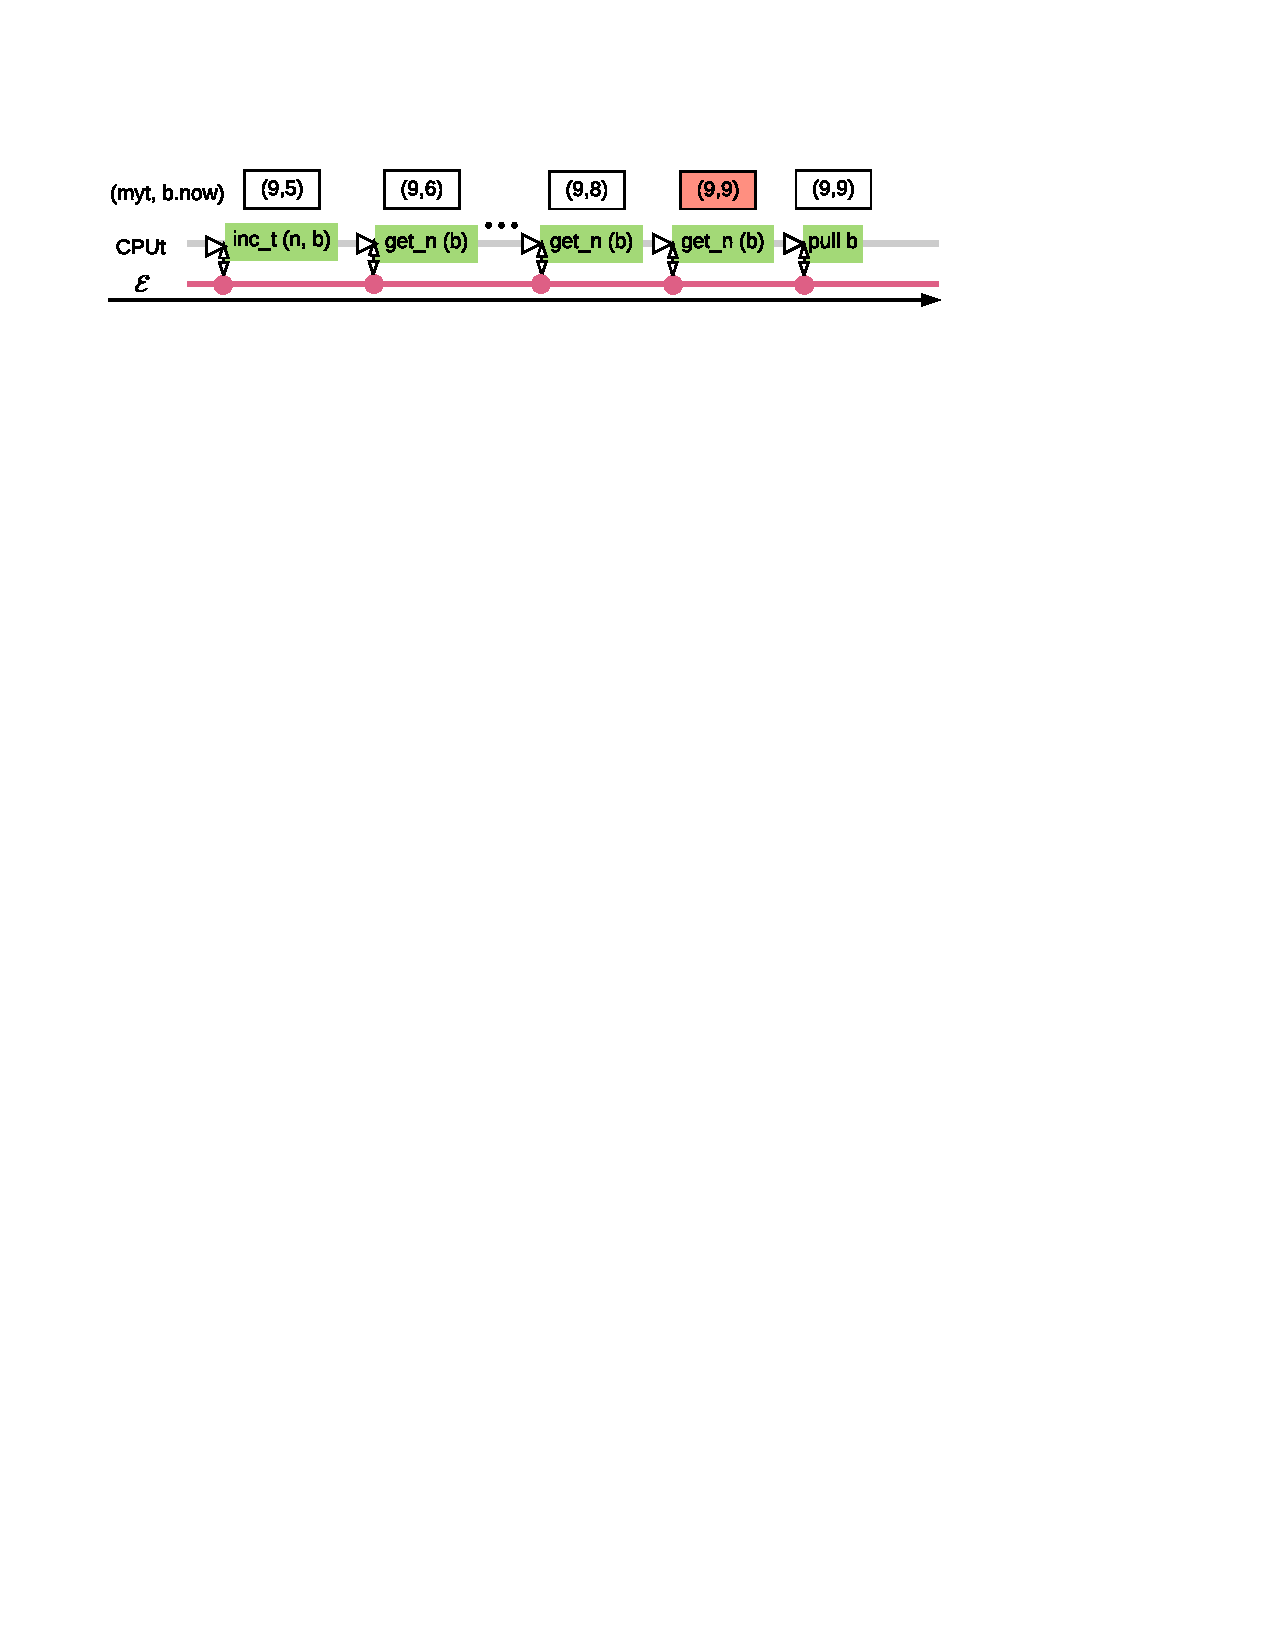
\includegraphics[scale=.9]{figs/ticket_log}
\]
\ignore{
The event list is as below:
$$[\intp,\event{t.inc\_ticket\ i},\intp,\event{t.get\_now\ i},\cdots,\intp,\event{t.get\_now\ i}]$$
}

To verify this ticket lock module,
we begin by 
introducing the extensions to the bottom layer interface,
then we write a
low-level functional specification for the lock implementation,
and finally we abstract this specification into a short
high-level description.


\noindent\textbf{Step 1 (introducing atomic memory operations for ticket lock in $L_\code{Preinit}$).}
Because the data structure $\comm{ticket\_lock}$ is used for communication
between concurrent CPUs, 
the bottom layer interface $L_\code{Preinit}$
has to define the globally visible events that can be generated. 
When writing these specifications in $L_\code{Preinit}$,  we can choose the type of events in any way, as long
as it is 
fine-grained enough that we can state all scheduling interleavings that
the code may encounter. In this case, we have events for the updates to
$\ticket$ and $\now$ and an event for reading the $\now$ value
for a lock $b$. Additionally, we make use of a natural number 
$n$\ignore{ and an event $\holdlock$}, which has no
operational significance and is explained below.
\[
\begin{array}{c}
L_\code{Preinit}.\Ev := \incticket(n, b) \mid \incnow(b) \mid \getnow(b)
\mid \push(b,bl) \mid \pull(b)
\ignore{\\
&  \mid &  \holdlock \mid \tshared (e : \mathsf{SharedMemEvent})}
\end{array}
\]%

To specify the meanings of the get and increment events, we define a replay
function $\replay_{\comm{ticket}} : Log \to \integer \to \integer\times \integer$. 
The definition is as one would expect:
$\replay_{\comm{ticket}}(\mathsf{nil}, b) = (0,0)$, each 
$\incticket(n, b)$ and $\incnow(b)$ event in the list increments
the first or second component of the pair, and other events are ignored.

We then specify the behavior of the primitives
of $L_\code{Preinit}$, which are implemented by the atomic instructions on the x86 architecture. 
For example, we implement the
fetch-and-increment $\mathsf{FAI\_ticket}$ primitive in a small 
assembly snippet, yielding the following specification:
%% Is this just assumed, or is it proved somewhere?
\begin{mathpar}
\inferrule{
 l_0 = l \cons \oracle(l) \\
  \replay_{\comm{ticket}}(l_0, b) = (i,j) \\
  l' = l_0 \cons c.\incticket(n, b)\\ 
}{
 \oracle, c \vdash  \spec_{\mathsf{FAI\_ticket}}([n, b], \regs, m, a, l, i, \regs, m, a, l')
}
\end{mathpar}%

In other words, this primitive queries $\oracle$, replays the result log to
compute the current state $i$ of {\tt ticket},
and then appends one
 event to the log. 
\ignore{The fact that we are
using an atomic memory instruction, and that such memory updates are
immediately visible to all CPUs, is reflected by the
primitive just adding a single event so there can be no unexpected
interleavings between CPUs. We add similar specifications for the
other operations, \eg, a $\sigma_{\mathsf{get\_now}}$ primitive whose
implementation is a memory read, and whose specification queries
$\oracle$ to get the new log $l_0$, appends $\getnow (b)$, and returns
$\mathsf{snd}(\replay_\mathsf{ticket}(l_0, b))$.}
The primitive set of $L_\code{Preinit}$ is defined as below:
\[
\begin{array}{rl}
L_\code{Preinit}.\primt := &\mathsf{FAI\_ticket} \mapsto \spec_{\mathsf{FAI\_ticket}}
\oplus \mathsf{inc\_now} \mapsto \spec_{\mathsf{inc\_now}} \\
&\oplus \mathsf{get\_now} \mapsto \spec_{\mathsf{get\_now}}\oplus  \push\mapsto \spec_{\push}
\oplus  \pull\mapsto \spec_{\pull}\\
& \oplus  \text{ sequential primitives}
\end{array}
\]%

\noindent\textbf{Step 2 (introducing low-level specifications for ticket lock in $L_\ttlockop$)}
In the next layer $L_\ttlockop$, 
we verify the implementation of the ticket lock based on
 $L_\code{PreInit}$. Since each lock is associated with a shared variable,
after the lock is acquired, it invokes $\pull(b)$ 
to update the shared memory at the corresponding location $b$
according to the log.
The bodies of the lock-acquire function $\acq$ and 
the lock-release function $\rel$ are verified as if they were 
sequential C programs. Uses of the lock primitives are handled
similarly to external function calls, by applying their
specifications. From the verifier's point-of-view, they are no 
different from code
that writes to a thread-local variable (namely, the log). 

However, we need some care to assign a good specification to these
functions. While $\rel$ is straightforward (just append the
$\push$ and $\incnow$ events to the log), 
$\acq$ contains a while-loop. To prove total correctness,
we would like to assign a specification which later can be proven
to terminate.

We define an auxiliary function $\comm{wait}$
(using recursion in Coq) describing the behavior of the first $k$
iterations of the loop: each time we query the environment
context $\oracle$, it generates its own
event and checks if CPU number $c$ is due to hold the
lock. The function is undefined (Coq {\tt None}) if we do not get the
lock within $k$ iterations.
\[
\begin{array}{lcl}
\mathsf{wait}(0, \oracle, c, b, l) & = &\text{undefined} \\
\mathsf{wait}(k+1, \oracle, c, b, l) & = & l', \text{ if $l'$ indicates next is $c$'s turn to get lock}\\
                       & &   \mathsf{wait}(k, \oracle, c,  b, (l' \cons c.\getnow(b))), \text{ otherwise} \\
                       & &  \text{where }l' = l \cons  \oracle(l)
\end{array}
\]%

We then define the semantics of the primitive by saying that it first
generates an $\incticket$ event and then loops
for some ``sufficiently'' large number $\calwait(l, c)$ of iterations.
\begin{mathpar}
\inferrule{
  l_0 = \mathsf{wait}(\calwait(l, c), \oracle, c, b,
  	l \cons \oracle(l) \cons c.\incticket(n,b)) \\
  (\bytelist,  \comm{invalid}) = \replay_\comm{get\_shared} (l_0, b) \\
  	m' = m \set{b: \bytelist}\\
  	a' = a \set{\perm{b}: \comm{valid}} \\
  	l'  = l_0 \cons c.\pull(b) \\
}{
 \oracle, c \vdash  \spec_{\acq\_\mathsf{low}}([n,b], \regs, m, a, l,\any, \regs, m', a', l')
}
\end{mathpar}%
Computations where $k$ reaches 0 are considered crashing, and our
ultimate theorem is about safe programs, so when proving that the C
code matches the specification we only need to consider finite
successful runs. It is easy to show that the C loop can match any of
those, since it can run any number of times.

To prove the \textbf{starvation-freedom} of ticket lock,
we have to know what number $\calwait(l,c)$ is sufficiently large.
Thus,  we need more information than just the two integers representing the lock
in memory. In this layer $L_1$, we introduce
a new  replay function:
\[
\replay_{\mathsf{wait\_q}} : Log \to  \mathsf{LockStatus} \times
 \mathsf{list}\ (\mathsf{CPU\_ID}\times\mathbb{N})
\]%
\adam{Why list instead of function}
\noindent{}This computes which CPU (if any) currently holds the log, and  a list of all CPUs that have started waiting for
the lock together with the natural number $n$ that
$\spec_{\acq}$ was given as an argument. The meaning of
$n$ is that once the CPU enters the critical section, it promises to take  at most $n$ steps before exiting. 
The replay function $\replay_{\mathsf{wait\_q}}$ is defined by going through the log
event by event; for example, $c.\incticket(n,b)$ appends $(c,n)$ to the list
of waiting CPUs.
Finally, in the proof we assume that the hardware scheduler is \emph{fair}, in the sense that there exists some 
constant $n_0$ such that any CPU will be rescheduled within $n_0$ steps. 
Then we can calculate maximum wait-time $\calwait(l, c)$ as $n_0$ times the sum of all the bounds $n$ for the CPUs waiting ahead of $c$ in the queue.

%% held'' to ``held'' and sets the ``time to finish'' $n_f$ to $n$. 
%% Assume the hardware scheduler is \emph{fair},
%% such that any CPU will be rescheduled within $n_0$ steps.
%% Thus, each event
%% generated by the CPU that holds the lock decrements the ``time to
%% finish'' counter $n_f$ (and resets the ``time until scheduled'' counter $n_s$ to be $n_0$),
%% while each event generated by some \emph{other} CPU decrements the
%% ``time until scheduled'' $n_s$. 
%% Let $\replay_{\comm{wait\_q}} (l) := (n_f, n_s, \any, q)$
%% for the current global log $l$.
%% By the fact that
%% $(n_f \le q[0].n)$ and 
%% $(n_s \le n_0)$, the \emph{maximum} wait-time $\calwait(l, c)$ can be calculated as below:
%% {\small
%% \[
%% \calwait(l, c) = n_0 + n_0 \times \sum_{n_i}
%% (i, n_i) \text{ for all CPU waiting before }c\text{ in }q
%% \]}

The primitive set of $L_\ttlockop$ consists of the lock related
primitives and the sequential ones inherited from $L_\code{PreInit}$:
\[L_\ttlockop.\primt := \acq \mapsto \spec_{\acq\_\mathsf{low}}
\oplus \rel \mapsto \spec_{\rel\_\mathsf{low}}
\oplus \text{ sequential primitives}\]
Thus, let $M_0 := \acq \mapsto \module_{\acq}
\oplus \rel \mapsto \module_{\rel}$,
we can build the concurrent layers as below:
\[
\forall \oracle, 
\ltyp{(L_\code{PreInit}, \oracle)}{\id}{M_0}{(L_\ttlockop, \oracle)}
\]%
Note that,
because the abstract state and the global log are identical
in both layers, the simulation relation is the identity relation $\id$.

\vspace{3pt}
\noindent\textbf{Step 3 (introducing atomic lock specifications in $L_\ttlock$)}
All the above details are irrelevant to clients using the lock, who only
need to know that they are allowed to get the lock as long as they
promise to release it within $n$ steps. We introduce a new layer $L_\ttlock$ to
suppress the details, where we use a simpler type of events and replay function.
\[
\begin{array}{l}
\replay_\mathsf{lock} : Log \to \mathbb{N} \times
\mathsf{LockStatus}\qquad
L_\ttlock.\Ev := \acq(n,b) \mid \rel(b,bl) \\
L_\ttlock.\primt := \acq \mapsto \spec_{\acq}
\oplus \rel \mapsto \spec_{\rel} \oplus \text{ sequential primitives}
\end{array}
\]%
The replay function computes which CPU (if any) currently holds the
lock and has a counter for how many more steps that CPU is allowed
to take. Again, this is computed event by event: if CPU $c$
generates the event $c.\acq(n,b)$, the high-level interpretation of the
log becomes $(n, \mathsf{held\_by}\ c)$ for lock $b$, and then 
 the counter decrements each time CPU $c$ takes a step. 
 If the counter
ever reaches $0$ the program is considered \emph{crashed}, so clients of the
lock need to prove that they respect the bound $n$ they
provided. (Typically this is easy, because most clients only carry out
some constant number of operations in the critical section.)

The specifications for the high-level lock and unlock primitives are
now very simple:
\ignore{We introduce a new abstract state $\lockstatus$,
which is a set of boolean saying
whether this CPU holds the lock (to express the precondition that you
can only get/release the lock if you are outside/inside the critical
section).  Thus, }$\acq$ and $\rel$ just query the environment context and then
introduce one more event.
\begin{mathpar}
\inferrule{
	l_0 = l \cons \oracle(l)\\
  (\bytelist,  \comm{invalid}) = \replay_\comm{get\_shared}(l_0, b) \\
  	m' = m \set{b: \bytelist}\\
  	a' = a \set{\perm{b}: \comm{valid}} \\
  	l' = l_0 \cons c.\acq(n,b) \\
}{
 \oracle, c \vdash  \spec_{\acq}([n,b], \regs, m, a, l,\any, \regs, m', a', l')
}
\\
\inferrule{
  m(b) = \bytelist \\
  a.\comm{perm}(b) = \comm{valid} \\
  a' = a \set{\perm{b}: \comm{invalid}} \\
  l' = l \cons \oracle(l) \cons c.\rel (b, \bytelist)
}{
 \oracle, c \vdash  \spec_{\rel}([b], \regs, m, a, l,\any, \regs, m, a', l')
}
\end{mathpar}

By having these primitives introduce only a single event, clients of the
lock code can treat the lock operations as completely \emph{atomic}; there is
no need to consider interleavings of the ``get lock'' execution
with events from other CPUs. In order to prove that this refinement
is sound, we must provide a function $f_{l1}$ from logs (and environment
contexts) at the lower layer to logs at the higher layer.  In this
case, $f_{l1}$ goes through the log and discards all events except for
$\pull$ and $\incnow$, which get mapped to $\acq$ and
$\rel$.
The function $f_{\oracle1}$ to convert the $\oracle$ 
and the simulation relation $R_1$ are both defined using $f_{l1}$.

The simulation proof
includes showing that $\spec_{\acq\_\mathsf{low}}$ is defined whenever
$\spec_{\acq}$ is, so we need to prove that the function
$\mathsf{wait}(\calwait(l, c), \oracle, c, b, l)$ returns a value. This is done
by computing a natural-valued termination metric for the log 
(in terms of
$\replay$) and showing that this decreases faster than $\calwait(l,c)$. In other words,
because our high-level specification of the lock is a total function,
proving that the implementation is correct includes a proof of
liveness. Thus,
\[
\forall \oracle, 
\ltyp{L_\ttlockop(c, \oracle)}{R_1}{\emptyset}{L_\ttlock(c,f_{\oracle1}(\oracle))}
\]%

This simulation proof is only between specifications.
By applying the vertical composition rule, \ignore{ (Lemma~\ref{lem:vertical})} we have:
\[
\forall \oracle, 
\ltyp{L_\code{PreInit}(c,\oracle)}{R_1}{M_0}{L_\ttlock(c, f_{\oracle1}(\oracle))}
\]


\subsection{MCS lock}
\label{sec:con:mcs}
\begin{figure}
\lstinputlisting [language = C, multicols=2] {source_code/mcs_lock.c}
\caption{MCS Lock Implementation}
\label{fig:exp:mcs_lock}
\hrulefill
\end{figure}

Ticket locks are inefficient in systems with very many processors (10
to 40, depending on workload~\cite{Boyd-wickizer12}), because every
CPU repeatedly reads the same memory location. As an alternative, we
implement the MCS algorithm~\cite{mcs91}. In this algorithm,
different CPUs competing for the lock each own one node of a
linked list in memory, which represents the queue of waiting CPUs. The
lock also contains a pointer to the tail of the list, which is shared
between all CPUs and has to be manipulated using atomic
compare-and-swap instructions. To take the lock, a CPU only
swaps the tail-pointer once, then modifies the next-pointer
of the previous node, and waits for the previous CPU to modify its own
node. 

% Sigh, I can't get this to look nice. 
\ignore{
\begin{figure}
\lstinputlisting [language = C, multicols=2] {source_code/mcs_lock.c}
%\vspace{-5pt}
\caption{Pseudocode of MCS-lock implementation.}
\label{fig:exp:mcs_lock}
%\vspace{-10pt}
\end{figure}
}


Compared to ticket locks, the MCS algorithm is more involved, since
the swap and modify events can be arbitrarily interleaved. For
example, the next-pointers in the list are not always valid and may
be updated in any order.  This makes it a good example, showing that
our verification methodology works for interesting concurrent
programs. Previously, this algorithm had only been proven correct
using pen-and-paper.

The verification strategy is very similar to the ticket locks,
and the structure provided by abstraction layers is even more helpful here. In the
memory operation layer, instead of calculating a pair of integers, the
replay function calculates a value of type 
$\integer \times (\mathsf{Map}\ \integer\ (\mathsf{bool}\times \integer))$, that is,
the value of the tail pointer and a finite map representing the list
nodes.  The rest of the proof does not need to concern itself
with a low-level memory model, and reasoning about the
replay function can be done similarly to reasoning about a pure
functional program.

The interface provided by the mid-level layer is then very similar to
the mid-layer $L_\ttlockop$ for ticket locks. Again, the state of the lock
can be summarized as a logical list of waiting CPUs and counters
bounding the number of operations they may perform. In order to capture the
additional complexity of next-pointers, we only need one more
component (a set of nodes). The proof of starvation freedom is quite
similar to the ticket lock, and the high-level interface $L_\ttlock$ is
identical to that exposed by the ticket locks.


\ignore{
\begin{figure}
\lstinputlisting [language = C, multicols=2] {source_code/mcs_lock.c}
\caption{MCS Lock Implementation}
\label{fig:exp:mcs_lock}
\end{figure}
}

\subsection{Device drivers}
\label{sec:con:device}
\citet{chen16} present a framework to allow interrupts
inside the kernel
with device drivers. The core idea is to treat device drivers of
each device as if they were running on a ``logical'' CPU dedicated to that device
and build a framework that systematically enforces the isolation among different
``devices'' and the rest of the kernel. The work has been successfully ported
into our setting relatively easily thanks to the fact that their event-based
 model is consistent with our interleaving machine model.


\subsection{Memory management}
\label{sec:con:mem}
\ignore{
The memory management of {\mCTOS} consists of  the
\emph{physical memory management} (4 layers), 
\emph{virtual memory management} (7 layers), and
\emph{shared memory management} (3 layers).
}

\ignore{
\begin{figure}
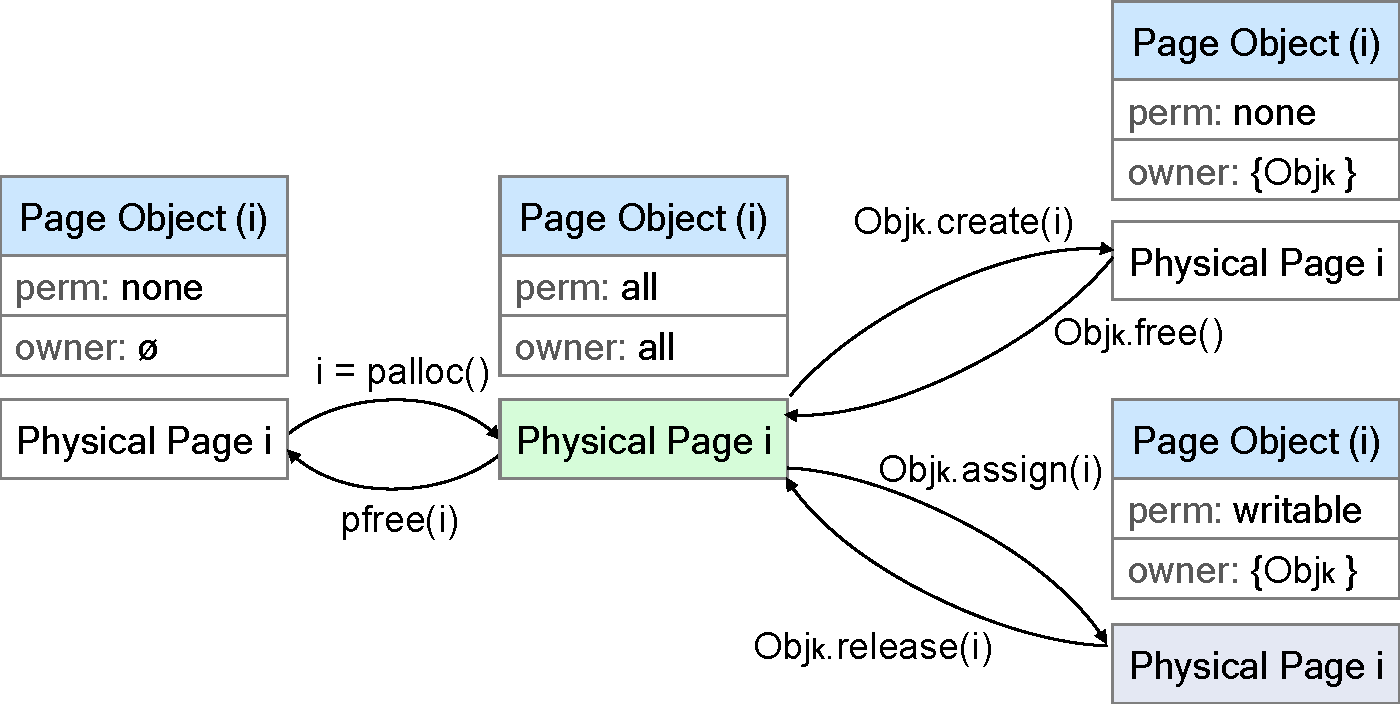
\includegraphics[scale=0.35]{figs/dynamic}	
\caption{The state transition of page object}
\label{fig:base:dynamic}
\vspace*{-14pt}
\end{figure}
}

As the page allocation table $\texttt{AT}$ is shared among different CPUs, 
we associate it with a lock $\texttt{lock\_AT}$.
The \emph{dynamic page allocator}
\texttt{palloc} (\cf Figure~\ref{fig:exp:palloc}) is then refined into an atomic object where
the \texttt{palloc} implementation is proved to satisfy an atomic interface,
with the proof that the lock is released within the bound.
Once the dynamic page allocator is introduced as
 an atomic object, the lock acquire and lock release 
for $\texttt{lock\_AT}$
are \emph{not allowed to be invoked} at higher layers. 
Thus, in this layered approach, it is not possible
that a thread holding a lock defined in a lower layer tries to acquire another lock
introduced in a higher layer, \ie, the order that a thread acquires different
locks is guided by the order that the locks are introduced in the layers.
This implicit order of lock acquisitions prevents \emph{deadlocks} in the
{\cCTOS} kernel.

\begin{figure}[t]
\lstinputlisting [language = C, multicols=2] {source_code/palloc.c}
\caption{Pseudocode of \texttt{palloc}}
\label{fig:exp:palloc}
\hrulefill
\end{figure}



\ignore{Another function of the physical memory management is to dynamically
track and bound the memory usage of each thread. A \emph{container}
object is used to record information for each thread (array \code{cn}
in Figure~\ref{fig:exp:palloc}); one piece of information tracked is the
thread's \emph{quota}. Inspired by the notions of containers and
quotas in HiStar~\cite{zeldovich06}, a thread
in {\mCTOS} is spawned with some quota specifying the maximum number
of pages that the thread will ever be allowed to allocate. As can be
seen in Figure~\ref{fig:exp:palloc}, \code{palloc} returns an error
code if the requesting thread has no remaining quota (lines~4 and~5), 
and the quota is decremented when a page is successfully allocated (line~17).
Quota enforcement allows the kernel to prevent a denial-of-service attack,
where one thread repeatedly allocates pages and uses up all available
memory (thus denying other threads from allocating pages). From a security
standpoint, it also prevents the undesirable information channel between 
different threads that occurs due to such an attack.}

\ignore{
\begin{figure}[t]
$$
\begin{array}{c|c}
\begin{array}{cc}
(a) &\
      \begin{array}{c}
			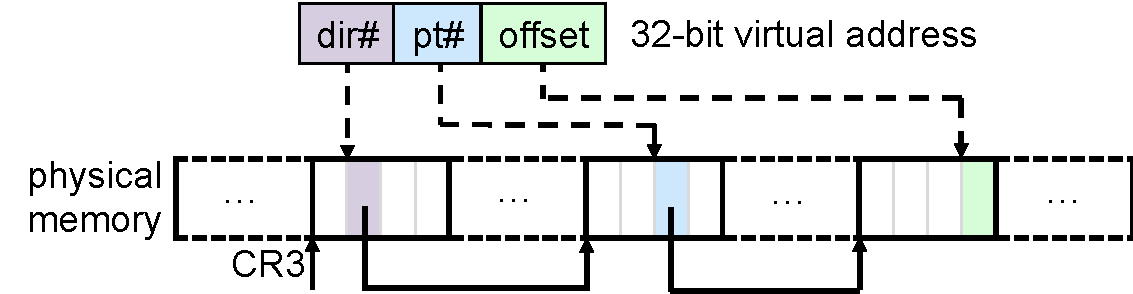
\includegraphics[scale=.3]{figs/mem_model_1} 
		\end{array}
\end{array}
& 
\begin{array}{cc}
(b) & 
\begin{array}{c}
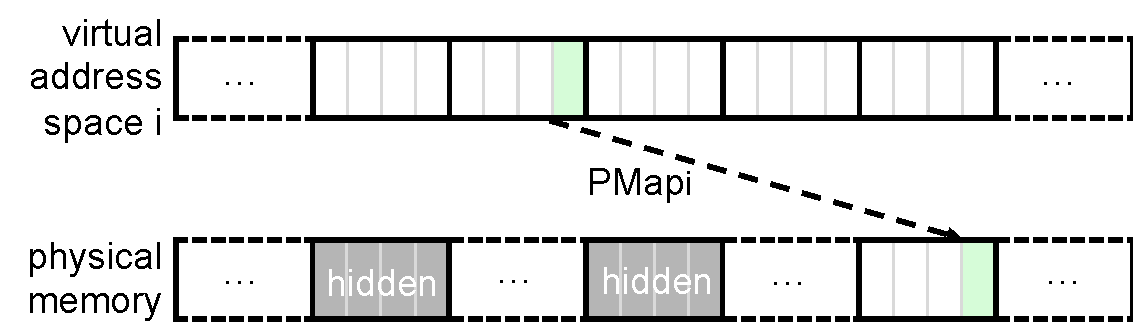
\includegraphics[scale=.3]{figs/mem_model_2}
\end{array}
\end{array}
\vspace*{-14pt}
\end{array}
$$
\caption{(a) Hardware MMU using two-level page map; (b) Virtual address space $i$ set up by page map $i$.}
\label{fig:spec:memmodel}
\hrulefill
\end{figure}}

\ignore{
\paragraph{Virtual memory management}
provides consecutive virtual address spaces on top of physical memory management.
\ignore{Because much of the code assumes that 
the memory management sets up the virtual address space properly,
initialization has been a sticking point.}
We proved not only that the primitives of virtual memory management
manipulate the page maps correctly,
but also that the \emph{initialization procedure} sets up the two-level page maps properly
in terms of the hardware address translation.


\begin{invariant}
\label{inv:virtual}
1) paging is enabled only after the initialization of virtual memory management;
2) the memory regions that store kernel-specific data must have the kernel-only 
permission in all page maps;
3) the page map used by the kernel is an identity map
4) the non-shared parts of user processes' memory are isolated (see 
Sec.~\ref{security}).
\end{invariant}


By Inv.~\ref{inv:virtual}, we show that it is safe to
run both the kernel and user programs in the virtual 
address space when paging is enabled.
In this way, memory accesses at higher layers
operate on the basis of
the high-level, abstract descriptions of address spaces
rather than concrete page directories and page tables stored in the memory
itself.}

\ignore{
\paragraph{Shared memory management} provides a protocol to share physical
pages among different user processes. 
It provides an infrastructure to map a physical page into multiple
processes' page maps (\ie, processes' address spaces).
We prove that the shared page can only be freed after 
all processes release their ownership of that page.}

\ignore{
Its verification makes use
of the ownership relation. 
For example, a user process $k_1$ can share its private physical page $i$
to another user process $k_2$ through the shared memory protocol,
and the owner set of page object $i$ will become
$\{\text{process object }k_1, \text{process object }k_2\}$.
}


\ignore{\subsection{Process management}


Process management  introduces the
\emph{abstract queue library} (4 layers),
\emph{thread management} (6 layers),
\emph{condition variable} (3 layers),
and \emph{IPC} module (2 layers).}

\ignore{\begin{figure}
\lstinputlisting [language = C, multicols=1] {source_code/enqueue.v}
\vspace{-5pt}
\caption{Specifications of local queue operations.}
\label{fig:exp:queue}
\vspace{-10pt}
\end{figure}}


\subsection{Shared queue library}
\label{sec:con:queue} 
Shared queue objects
are widely used in concurrent kernels, \eg, as buffers for producer/consumer,
as the list of threads in a scheduler, {\etc}
In previous work~\cite{lili16},
due to the lack of layering support,
the verification of any shared object
has to inline the lock implementation
and duplicate the lock-related proofs.
In \cCTOS, we illustrate how we utilize concurrent
abstraction layers to simplify the verification of a shared queue object 
implemented with fine-grained \emph{spinlocks}, which is introduced by the layer $L_\ttlock$ and passed to the layer
$L_\pkctxop$.

\ignore{The specification of a shared queue object should provide a high level abstract
interface by hiding all the low level details,
to ease the verification of programs using the object.
However, the large gap between this high level abstract specification
and the low level efficient implementation makes the verification of the shared queue object
itself extremely challenging.
Furthermore,}

Our shared queue library abstracts the queues implemented as \emph{doubly-linked lists}
into \emph{abstract queue states} (\ie, Coq lists).
The local {\it enqueue} and {\it dequeue} operations
are specified over the abstract lists.
As usual, we associate each shared queue with a lock.
The atomic interfaces for shared queue operations are represented by
queue events ``$c.\mathsf{enq}(i,e)$" and 
$``c.\mathsf{deq}(i)"$,
which can be replayed to construct the shared queue. 
For instance, starting from an empty initial queue,
the resulting queue constructed from
the log of the following interleaving
is $[2,5]$, and the last dequeue operation returns 3.
\ignore{ 
if the current local log of $i$'th shared queue is
$[\intp,\event{t_0.enQ\  i\ 2},\intp,\event{t_0.deQ\ i}]$,
and the event lists generated by the \emph{environment context} at two {\intptext}s are
$[\event{t_1.enQ\  i\ 3},\event{t_1.enQ\  i\ 4}]$ and
$[\event{t_1.enQ\  i\ 5}]$, respectively,
then the complete logical log for the shared queue $i$ is:}
\[
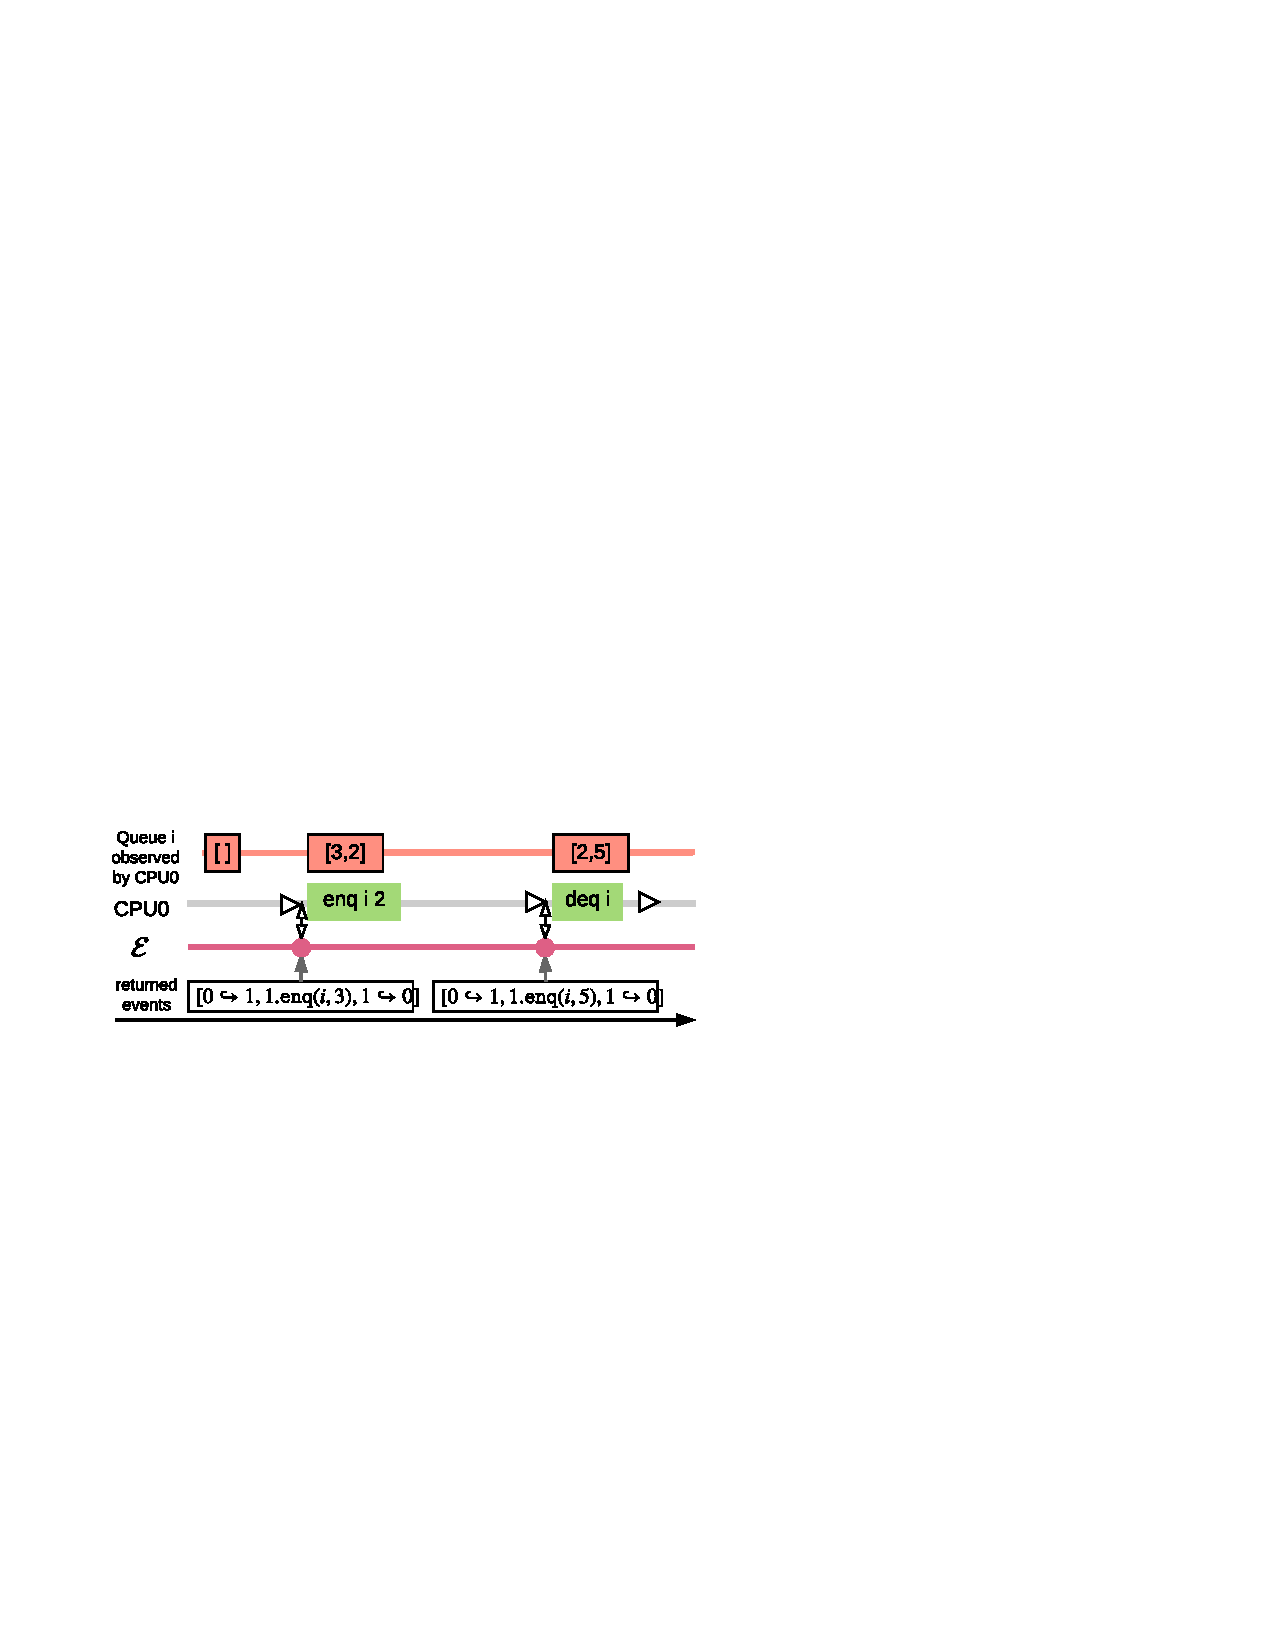
\includegraphics[scale=.9]{figs/queue_log}
\]
\ignore{
$$[\event{t_1.enQ\  i\ 3},\event{t_1.enQ\  i\ 4},\event{t_0.enQ\  i\ 2},\event{t_1.enQ\  i\ 5},\event{t_0.deQ\ i}]$$
}

\ignore{Thus, by replaying the log, the shared queue state is calculated as $[4,2,5]$,
and the last atomic dequeue operation returns 3.}

The certified layers for the shared queue object
are built as the following steps.

\noindent\textbf{Step 1 (intermediate layer $L_\pqintro$)} 
Figure~\ref{fig:exp:dequeue} shows
the implementation of a dequeue operation $\deq$ in terms of a doubly linked
list.
It first acquires the spinlock associated with queue $i$
(via the auxiliary function $\qloc$),
then invokes the local dequeue operation $\deq\comm{\_t}$
and releases the lock.
Instead of directly verifying the function $\module_{\deq}$
with fine-grained locking in one shot, we do it over
multiple layers.
We first introduce an intermediate function
$\module_{\deq\comm{\_t}}$ (\cf Figure~\ref{fig:exp:dequeue}), which contains
the code that performs the local dequeue operation but assumes that
the corresponding lock is held.
Verification of the function $\module_{\deq\comm{\_t}}$ is now much
simpler because it can be treated as a sequential program.
For this purpose, we introduce a new layer interface $L_\pqintro$ as follows:
(1) introduce abstract states $abs_\comm{tcbp}$ and $abs_\comm{tdqp}$;
(2) define a simulation relation $R_{2}$ between the new abstract states
and the concrete doubly linked list in memory;
and (3) prove the simulation between
$\module_{\deq\comm{\_t}}$ and its specification
$\spec_{\deq\comm{\_t}}$.

\ignore{Suppose the underlying layer interface is:
$$L_1.P = \acq \mapsto \spec_{\acq}
	\oplus \rel \mapsto \spec_{\rel}$$}
	
The newly introduced $(abs_\comm{tdqp}: \integer \partf 
\comm{List\ }\integer)$ is a partial map from \emph{queue index}
to the \emph{abstract queue}, which is represented as
a list of indices to thread control blocks (\ie, $\comm{tcb}$).
The specification $\spec_{\deq\comm{\_t}}$ is defined as below:
\begin{mathpar}
\inferrule{
 \replay_\comm{lock\_status} (l,\qloc(i)) 
 = \comm{held\_by}\ c \\
 (a', res) =
 (\comm{if}\ a.\comm{tdqp} (i) = r\cons q 
\ \comm{ then }\  (a.\comm{tdqp}\set{i: q}, r)
 \ \comm{ else}\ (a, -1))
}{
 \oracle, c \vdash  \spec_{\deq\comm{\_t}}([i],\regs, m, a, l,res, \regs,  m, a', l)
}
\end{mathpar}
The  simulation relation 
$R_{2} (s_2, s_3)$ between $L_\pkctxop$ and $L_\pqintro$
%$R_{12}: L_1.\comm{state}\rightarrow L_2.\comm{state} \rightarrow \comm{Prop}$
is:

\begin{itemize}
\itemsep0em
\item Memory and abstract states are the same, except for $\comm{tcbp}$,  $\comm{tdqp}$.
\ignore{,
$abs_\comm{tcbp}$,  and $abs_\comm{tdqp}$}
\item There is no permission for $\comm{tcbp}$
and $\comm{tdqp}$ in $s_3.m$.
\item There exist functions $f_\comm{tcbp}$
and $f_\comm{tdqp}$, which map the thread control blocks and the doubly linked list in $s_2.m$ to $s_3.a$.
\item There exists a function  $f_{l2}(s_2.l) = s_3.l$,
which maps the events $c.\acq(n,\qloc(i))$ and $c.\rel(\qloc(i), bl)$
to $c.\acq_q(n,i)$ and $c.\rel_q (i, f_\comm{tdqp}(bl))$,
respectively.
\item  As for environment context,  $f_{\oracle 2}$  can be defined using $f_{l2}$.
\end{itemize}
\ignore{
as:
\begin{small}
\[
f_{\oracle 2} (\oracle) (l, c, b)=
\begin{cases}
f_{l2} (\oracle(l', c, b)) & \text{if } \exists l', f_{l2}(l') = l \wedge \reach(\oracle, c, l')\\
[] & \text{otherwise}
\end{cases}
\]
\end{small}

Note that since $\oracle$ represents the strategy of the environment
context, not all the logs are \emph{reachable} starting from the empty log.
This reachable set is defined as:
\begin{small}
\begin{mathpar}
\inferrule{ }
{
\reach(\oracle, c, [])
}
\and
\inferrule{\reach(\oracle, c, l) \\ b = \comm{block} (e)}
{
\reach(\oracle, c, c.e \cons \oracle(l,c,b) \cons l)
}
\end{mathpar}
\end{small}
If both $l$ and $l'$ are reachable logs from $\oracle$,
we can prove that $f_{l2} (\oracle(l, c, b)) =f_{l2} (\oracle(l', c, b))$. Therefore,  $f_{\oracle2}$ is well-defined.}

Let $L_\pqintro.\primt := L_\pkctxop.\primt \oplus \deq\comm{\_t} \mapsto \spec_{\deq\comm{\_t}}$ 
and
$M_2 :=  \deq\comm{\_t} \mapsto \module_{\deq\comm{\_t}}$.
We build the concurrent abstraction layer:
\[
\forall \oracle, 
\ltyp{L_\pkctxop(c,\oracle)}{R_2}{M_2}{L_\pqintro(c,f_{\oracle 2} (\oracle))}
\]
\ignore{This simulation is proved
by showing that $s_2.l$ is reachable from $\oracle$
and that $f_{l2}(s_2.l) = s_3.l$ always holds.
\david{I don't follow this sentence, it seems unnecessary.}}

\begin{figure}[t]
\lstinputlisting [language = C, multicols=2] {source_code/dequeue.c}
\caption{Pseudocode of dequeue implementation.}
\label{fig:exp:dequeue}
\hrulefill
\end{figure}

\noindent\textbf{Step 2 (atomic specification $L_\pqueue$)}
Next we verify the actual function $\module_{\deq}$ that wraps
$\module_{\deq\comm{\_t}}$ with the lock primitives.
We build a new layer interface $L_\pqueue$ that merges the two lock events
$\acq$ and $\rel$ into a single event $\deq$,
by showing that the dequeue operation, protected with spinlocks,
satisfies the atomic specification $\spec_{\deq}$ defined as:
\begin{mathpar}
\inferrule{
 l_0 = l \cons \oracle(l) \\ 
 \replay_\comm{get\_queue} (l_0, i) 
 = q \\
res =
 \comm{if}\ (q = r\cons q') 
\ \comm{ then }\  r
 \ \comm{ else}\ -1 \\
  l' = l_0 \cons c.\deq(i)
}{
 \oracle, c \vdash  \spec_{\deq}([i],\regs, m, a, l,res, \regs,  m, a, l')
}
\end{mathpar}
, where $\replay_\comm{get\_queue}$
calculates the queue of CPUs waiting for the lock.

The simulation relation 
$R_{3}$ between $L_3$ and $L_4$ is trivial,
except for the log function $f_{l3}$.
It drops the event $c.\acq_q(n,i)$
and maps the event $c.\rel_q(i, q)$
to $c.\deq(i)$. Thus, the function $f_{\oracle 3}$ to convert
$\oracle$ can be defined using $f_{l3}$.
\ignore{
\begin{itemize}
\itemsep0em
\item The memory and abstract state are the same, except for  $abs_\comm{tdqp}$.
\item $s_3.a.\comm{tdqp} (i) = 
L_4.\replay_\comm{get\_queue} (s_4.l, i) $,
which means that the queue constructed from
$s_4.l$ is equal to the queue in $s_3.a$.
\item There exists a function $f_{l3}(s_3.l) = s_4.l$,
which omits the event $c.\acq_q(n,i)$
and maps the event $c.\rel_q(i, q)$
to $c.\deq(i)$. 
Constructing  $f_{\oracle 3}$ from $f_{l3}$ is similar to
the ticket lock example.
\end{itemize}
\ignore{Therefore, we can define the function $f_{\oracle 1}$ for environment context:}}
Let $L_\pqueue.\primt := L_\pqintro.\primt \oplus \deq \mapsto \spec_{\deq}$ 
and
$M_3 :=  \deq \mapsto \module_{\deq}$.
We build the concurrent abstraction layer:
\[
\forall \oracle, 
\ltyp{L_\pqintro(c, \oracle)}{R_3}{M_3}{L_\pqueue(c, f_{\oracle 3} (\oracle))}
\]
Vertical composition then yields the desired result:
\[
\forall \oracle, 
\ltyp{L_\pkctxop(c,\oracle)}{R_3\cdot R_2}{M_2 \oplus M_3}{L_\pqueue(c,f_{\oracle 3} \cdot f_{\oracle 2}(\oracle))}
\]

\subsection{Thread management}
\label{sec:con:thread}

\begin{figure}[t]\centering
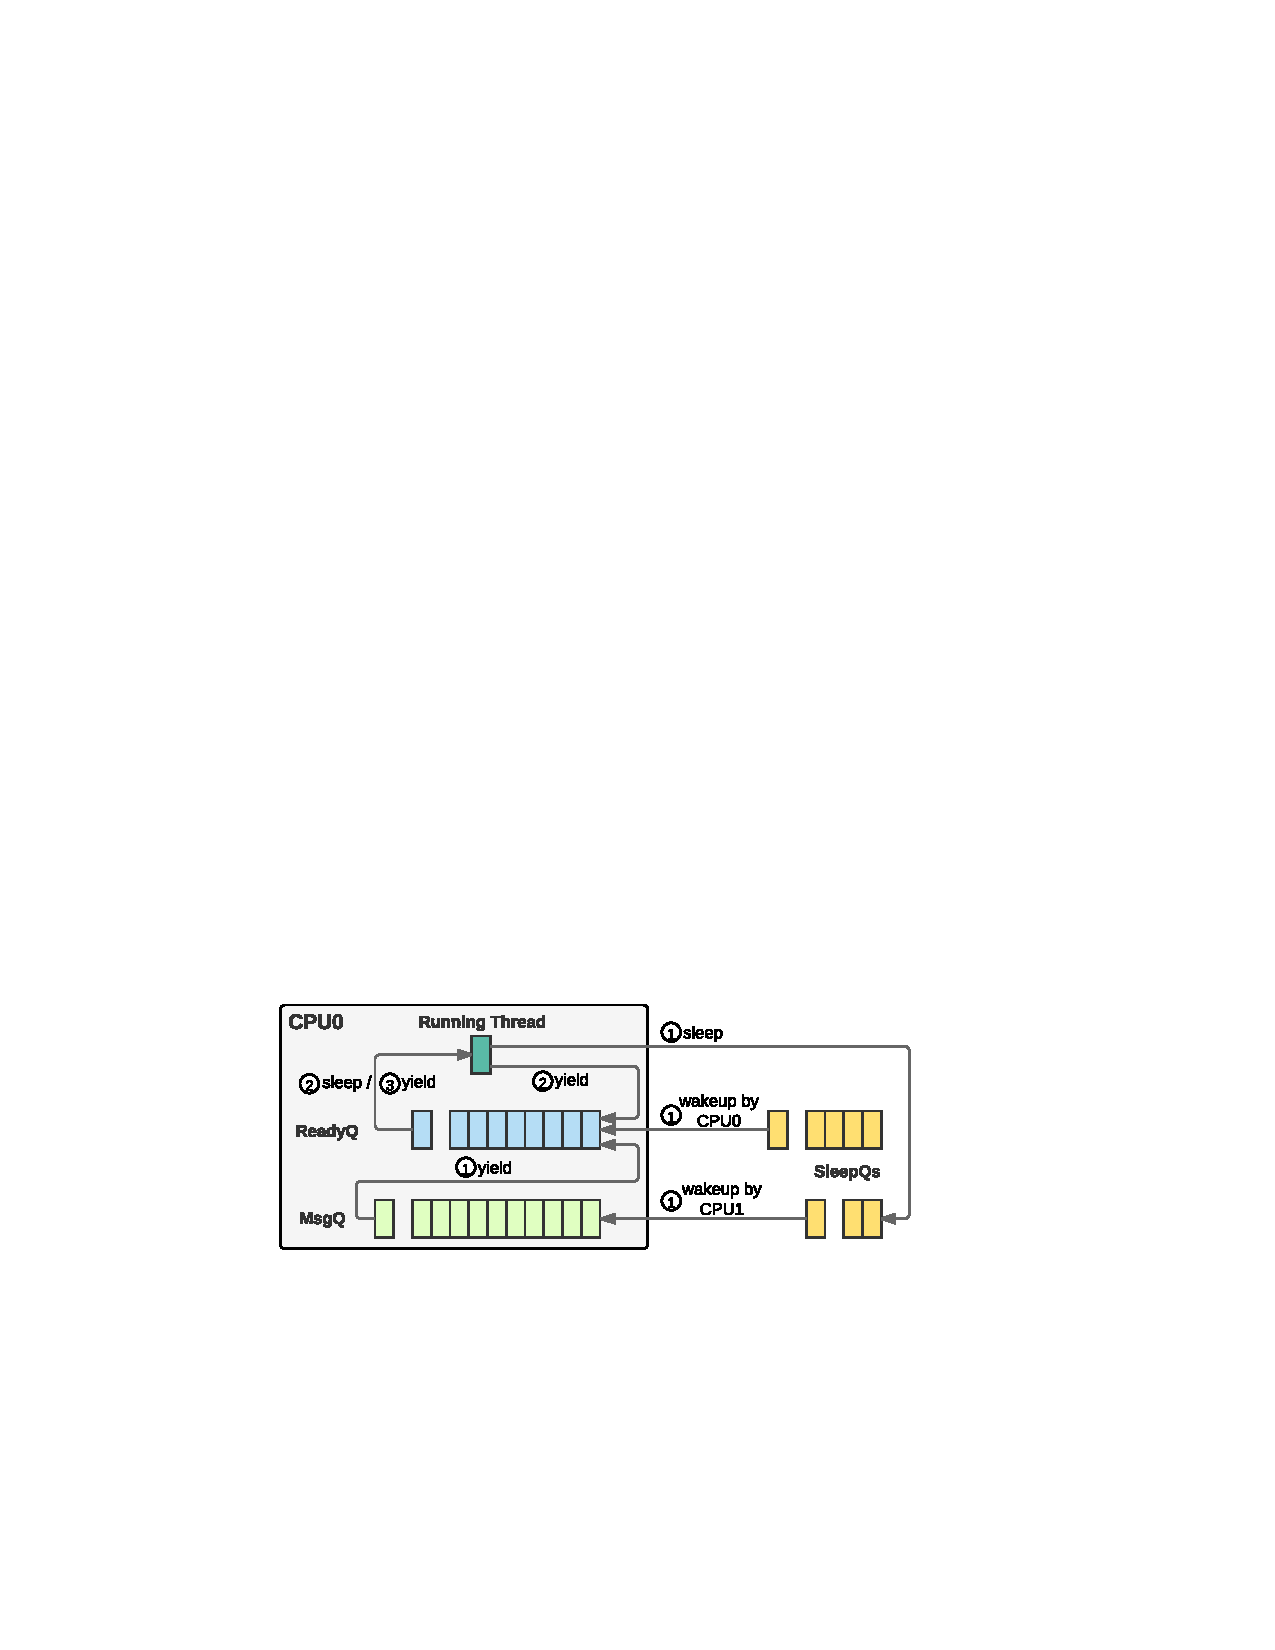
\includegraphics[scale=1.4]{figs/scheduler} 
\caption{Scheduling procedures of \texttt{yield}, \texttt{sleep},
and \texttt{wakeup}.\adam{seems not helpful}}
\label{fig:exp:fig:scheduler}
\hrulefill
\end{figure}

The thread management of \cCTOS{}
provides three primitives
(\ie, $\yield$, $\sleep$, and $\wakeup$)
for  thread scheduling and explicit synchronization between threads
(\cf Figure~\ref{fig:exp:fig:scheduler}). 
Each CPU has a \emph{private ready queue} ReadQ
and a \emph{shared message queue} MsgQ.
The context CPUs can insert threads to the current CPU's pending queue.
The {\cCTOS} kernel also provides a set of \emph{sleeping queues} SleepQs, which are
shared among all CPUs.
As shown in Figure~\ref{fig:exp:fig:scheduler},
the \code{yield} primitive moves a thread from
the pending queue to the ready queue
and then switches to the next ready thread.
The \code{sleep} primitive simply adds the running thread to the sleeping
queue and runs the next ready thread.
The \code{wakeup} primitive contains two cases.
If the thread to be woken up belongs to the current CPU,
then the primitive adds the thread to its ready queue.
Otherwise, \code{wakeup} adds the thread to the pending queue of the CPU it belongs to.
Except for the ready queue,
all the other thread queue operations are protected by \emph{fine-grained} locks.

\ignore{
\begin{figure}[t]
\lstinputlisting [language = C, multicols=2] {source_code/thread_management.c}
\caption{Implementation of the Scheduler Module}
\label{fig:exp:scheduler}
\hrulefill
    \afterpage{\FloatBarrier}
\end{figure}}

Verification of such scheduling primitives is extremely challenging.
Previous work either directly models the abstract scheduler primitives at a high level
(\eg, simple switch in the thread ID~\cite{xu16})
or verifies the scheduler functions with a low level small-step semantics
(\eg, saving and restoring the register set) \cite{dscal15}.
Both approaches have severe limitations. 
\adam{Compare bedrock 15' paper}
The first approach provides no formal connection
between the specification and underlying C and assembly implementation of those
scheduler functions. In the second approach, the specifications are too low level to
be useful in verifying the actual programs calling these primitives. Furthermore,
some portion of scheduler functionality is implemented in assembly (\eg, context switch).
Thus the semantics does not satisfy the C calling convention, meaning that it 
is impossible to reason about programs calling these assembly functions at the C level.

In this section, we build concurrent layers for the assembly part
of a scheduler in a small-step manner, but later lift the specifications
to big-step ones satisfying the C calling conventions. 
This allows us to perform \emph{thread-local} reasoning of programs
at the C level, where the proved properties of each thread can be linked formally
to obtain a global claim about the whole set of threads running on a processor.
To the best of our knowledge, this is the first attempt \adam{Compare bedrock 15' paper}
to support modular verification
of multi-threaded applications with explicit synchronization using verified
low level scheduler primitives.

\noindent\textbf{Step 1 (assembly-level specification $L_\pthread$)} 
Figure~\ref{fig:exp:sched} shows the implementation
of selected scheduling functions.
The $\yield$ function first polls a pending
thread from the per-CPU message queue
(\ie, $\comm{msgq}(c)$),
then selects the next running thread
from the CPU-local ready queue
(\ie, $\comm{rdq}(c)$),
and finally switches the kernel context.
The $\sleep$ function is similar: it
puts the current running thread
on the sleeping queue (\ie, $\comm{slpq}(q)$) and
then context switches.
The $\wakeup$ function moves the head of the sleeping queue
into the corresponding CPU's pending queue.
The context switch function $\mathsf{kctx\_switch}$
is exactly the same with the sequential setting (\cf Figure~\ref{fig:exp:cswitch}), which 
saves the current thread's kernel context (including the 
\emph{stack pointer}),
and loads the context of the target thread.
Note that this context switch function can only be implemented at the assembly level
and its specification does not satisfy the C calling convention.
To verify these low level scheduler functions, we introduce an
assembly-style concurrent layer interface $L_\pthread$.
\begin{figure}[t]
\lstinputlisting [language = C, multicols=2] {source_code/scheduling.c}
\caption{Pseudocode of scheduling implementation.}
\label{fig:exp:sched}
\hrulefill
\end{figure}


At layer $L_\pthread$, we introduce three new events
$c.\yield$, $c.\sleep(i)$, and $c.\wakeup(i)$,
which map to $L_\pqueue$'s events
$c.\deq(\comm{msgq}(c))$,
$c.\enq(\comm{slpq}(i))$,
and $c.\enq(\comm{msgq}(c))$, respectively.
Since the mapping is one-to-one, the transformation functions for
the log ($f_{l4}$) and environment context ($f_{\oracle4}$)
can be defined trivially.
The specifications of $\yield$ and $\sleep$
are defined as follows:
\begin{mathpar}
\inferrule{
l_0 = l \cons \oracle (l) \\
\replay_{\comm{sched}} (l_0, c) = (tid, tdqp, tcbp) \\
a' = a\set{\comm{kctxp}(tid) : \regs[\comm{ra},
\comm{ebp}, \comm{ebx}, \comm{esi}, \comm{edi}, \comm{esp}]} \\
l' = l_0 \cons c.\yield/c.\sleep(i) \\
\replay_{\comm{sched}} (l', c) = (rtid, \any, \any) \\
\regs' = (\regs\leftarrow a.\comm{kctxp}(rtid) )\set{\code{eax}:0} 
}{
 \oracle, c\vdash_{\comm{Asm}}  \spec_{\yield/\sleep}([]/[i],\regs, m, a, l,\any, \regs',  m, a', l')
}
\end{mathpar}%
The abstract states $\comm{tid}$,
$\comm{tdqp}$, and $\comm{tcbp}$
are hidden at $L_\pthread$, since they can always be reconstructed
by the replay function $\replay_{\comm{sched}}$ given the current log.
The replay function $\replay_{\comm{sched}}$
is defined inductively.
Here we only present the case for the $\sleep$ event:
\begin{mathpar}
\inferrule{
\replay_{\comm{sched}} (l, c) = (tid, \comm{tdqp}, \comm{tcbp}) \\
\comm{tdqp} (\comm{rdq}(c)) = r\cons q \\
\comm{tdqp} (\comm{slpq}(i)) = q' \\
\comm{tdqp}'  = \comm{tdqp}
\set{\comm{rdq}(c): q}
\set{\comm{slpq}(i):q'\cons tid}\\
\comm{tcbp}'  = \comm{tcbp}
\set{tid: \comm{SLEEP}}
\set{r:\comm{RUN}}
}{
\replay_{\comm{sched}} (l \cons c.\sleep (i), c) = (r, \comm{tdqp}', \comm{tcbp}') 
}
\end{mathpar}%
\noindent\textbf{Step 2 (multi-threaded machine $\TAsm$)} 
The  layer interface $L_\pthread$ is defined for the whole
set of threads for CPU $c$ and does not support thread-local reasoning.
Ideally, we would like to reason about each thread running on the CPU 
locally, and later formally combine the reasoning to obtain a global
property for the full set of threads.
To support this, we need a machine model that gives semantics to
a partially-composed set of threads.

Let $T_c$ denote the whole set of threads running over CPU $c$.
From the assembly machine $\LAsm(L_\pthread(c,\oracle))$, we construct a new 
multi-threaded \emph{partial} machine $\TAsm$
and instantiate it with a layer interface $L_\phthread$.
The result machine 
$\TAsm(L_\phthread(c), A)\langle \oracle \rangle$ is 
parameterized over an active thread set $A \subseteq T_c$
and can be instantiated into a regular machine for
an environment context $\oracle$.
The machine state of $\TAsm$ is defined as $s:=(\tid, f_\regs, m, f_a, l)$.
Here, $\tid$ is the current thread ID, and
$f_\regs$ and $f_a$ are partial functions
from IDs of threads in $A$ to a register set $\regs$
and a per-thread abstract state $a$, respectively (\ie,
we divide the register set and the abstract state
into separate ones for each thread).
The relation between abstract states
can be easily defined, but the relation of the register set between $L_\pthread$ and $L_\phthread$ is non-trivial.
For the currently running thread, its local register set ($s_6.f_\regs(s_6.\tid)$) is equal
to the register set of $L_\pthread$ ($s_5.\regs$).
For other threads of $L_\phthread$, the local register set is equal
to the corresponding saved kernel context of $s_5$ for the registers
$[\comm{ra}, \comm{ebp}, \comm{ebx}, \comm{esi}, \comm{edi}, \comm{esp}]$.
In other words, the register set is decomposed in a way such that the $\regs$ of the
currently running thread is equal to the machine's register set, while the $\regs$ of
other threads is equal to the corresponding kernel context saved by context switch.

\ignore{
However, $m$ is using
the CompCert memory model \cite{leroy08},
which is not compositional \ronghui{reference here?Tahina?}.
We introduce a new \emph{algebraic memory
model} to make the CompCert memory model
modular (\cf Sec.~\ref{sec:comp} for more details).
Two machines are composable only if they have the same
logical log $l$.
}

For instructions and primitives that do not change the current thread
ID, their semantics are lifted from $L_\pthread$ to $L_\phthread$
by operating on the state $(f_\regs(\tid), m, f_a(\tid), l)$.
The scheduling functions (which may change the thread ID to a thread outside of $A$)
are part of the definition of $\TAsm$
and may trigger environment steps by generating events
that will switch control to a thread outside of $A$.
For instance,
the $\yield$ operation of $\TAsm$
will generate a $c.\yield$ event that will switch control to the next thread
and set the machine's $\tid$ accordingly.
If the new thread is in $A$,
then the $\TAsm$ machine will simply keep running local steps of the new thread.
If the new thread is outside of $A$,
then the machine will take environment steps
until the log indicates that control switches back to  $A$.

When $A$ is the entire thread set $T_c$ of core $c$,
it will never switch to environment threads and
we have the following refinement:
\begin{lemma}
$\forall \oracle\ ,~
\LAsm(L_\pthread(c,\oracle)) 
\refines
\TAsm(L_\phthread(c), T_c)\langle \oracle \rangle$%
\label{thread_composition}
\end{lemma}

However,
the partial machine $\TAsm$ can also be decomposed using the linking operator $\Join$,
which enables thread-local reasoning:
\begin{lemma}
$
\TAsm(L_\phthread(c), T_c)
\Refrel_\id
\bigJoin_{t \in T_c}
\TAsm(L_\phthread(c), \{t\})
$
\label{thread_compose}
\end{lemma}

%-----------------------------
\ignore{
For scheduling functions (which may change the thread ID to one for a thread not in $A$),
it may trigger the environment step by querying the environment
context $\oracle_T$, which capture the behavior of \emph{inactive} threads (\ie, the threads in $T_c - A$).

We define the specifications of scheduling functions using $\oracle_T$.
For example, the $\yield$ primitive at $L_6$ is specified as:
\begin{small}
\begin{mathpar}
\inferrule{
l_0 = l \cons \oracle (l) \\
(l', \tid') =  \comm{yield\_back}
(A, \oracle_T, l_0 \cons c.\yield) \\
f_\regs' = f_\regs\set{\tid': 
\text{undefined value except for }[\comm{ra},
\comm{ebp}, \comm{ebx}, \comm{esi}, \comm{edi}, \comm{esp}]}
}{
 A, \oracle_T, \oracle, c\vdash_{\comm{Asm}}  \spec_{\yield'}([],\tid,f_\regs, m, f_a, l,\any, \tid', f_\regs',  m, f_a, l')
}
\end{mathpar}
\end{small}%

Note that $\yield$ changes the $\tid$ to $\tid'$.
After that, the execution operates on
the state $f_\regs'(\tid')$ and $f_a(\tid')$.
When $\tid'$ is different from $\tid$, this simulates the behavior of context switch
within the active thread set $A$. 
If the active thread set $A$ is $T_c$, we have:
}

\ignore{
If the active thread set $A$ is the whole
thread set $T_c$, we have:

Then, we can prove the simulation
relation:
\begin{lemma}[$\LAsm$ refines $\TAsm$]
\label{thread_composition}
{\small
\[
\forall \oracle,~
\LAsm(L_5(c,\oracle)) 
\refines
\TAsm(L_6(c,\oracle, T_c, \any))
\]}%
\end{lemma}



\begin{lemma}[CPU-local machine refines multi-thread machine]
{\small
\[
\forall M~ \oracle, 
\sem{ }{M}L_5(c,\oracle) \Refrel_{R_5} 
\sem{}{M}L_6(T_c, \oracle)
\]}
\label{whole_thread_composition}
\end{lemma}}

\ignore{
\textbf{Proof sketch}:
For whole thread set,
the environment context only carries
the information of the context CPUs.
Thus, $\oracle_{T_c} = \oracle$.
For the simulation relation $R_5(s_5,s_6)$, 
the only non-trivial part is the relation
for register set function $s_6.\regs p$.
For the current thread,
$s_6.\regs p(s_6.\tid)= s_5.\regs$.
For other threads,
the register set of $s_6$ is equal
to the kernel context of $s_5$
for the register list
$[\comm{ra},
\comm{ebp}, \comm{ebx}, \comm{esi}, \comm{edi}, \comm{esp}]$.
\ignore{
which is defined as:
1) ;
and 2)$\forall i \neq s_6.\tid,
s_6.\regs p(i)= s_5.a.\comm{kctxt}$.}
}
%-----------------------------

\noindent\textbf{Step 3 (thread-local layer interface $L_\lthread$)} 
Finally, we introduce a per-thread layer interface $L_\lthread$, which is parameterized
over a single active thread $t\in T_c$.
Thus, $\yield$ always yields back to itself,
and there is no longer any ``internal'' low level context switch among active threads.
Thus, we obtain the following big-step specification of $\yield$ that actually
satisfies the C calling convention:
\begin{small}
\begin{mathpar}
\inferrule{
l_0 = l \cons \oracle (l)\\
(l', \tid) =  \comm{yield\_back}
(\tid, \oracle, l_0 \cons c.\yield)
}{
 \tid, \oracle, c, \oracle \vdash  \spec_{\cyield}([],\regs, m, a, l,\any, \regs,  m, a, l')
}
\end{mathpar}
\end{small}%
Here, the auxiliary function $\comm{yield\_back}$ 
specifies the behavior of repeatedly querying the environment context
$\oracle$ until the control flow yields back to the thread of interest $\tid$.
It appends all the events triggered by the inactive threads to the log.
To prove termination-sensitive contextual refinement,
we prove that $\comm{yield\_back}$ actually terminates,
by showing that the scheduler is \emph{fair} and every running
thread gives up the CPU within a finite number of steps.

On top of this thread-local machine $\LAsm(L_\lthread(c, t, \oracle))$,
we can reason about a thread's program 
locally at the C level by building per-thread layers.
We show that $L_\phthread$ for a single thread is refined by $L_\lthread$:
\[ \TAsm(L_\phthread(c), \{t\})\langle \oracle \rangle \Refrel \LAsm(L_\lthread(c, t, \oracle)) \]
%

% ------------------------------------------------------------------
% Let's not talk about linking partial machines here
\ignore{
By Lemma~\ref{lemma:mono},
per-thread layers can be composed using
``$\Join$", and propagated down to the $L_6$ machine.
Once the layers are composed for the full thread set $T_c$, we can apply Lemma~\ref{thread_composition}
to transfer the guarantee down to $L_5$
and link with per-CPU layers.
}
% ------------------------------------------------------------------

\subsection{Synchronized IPC module}
\label{sec:con:ipc}
We have implemented and verified a single-copy
inter-process communication (IPC) protocol using condition variables
and the FIFO Blocking Bounded Queue.
Additionally, we have verified a
zero-copy IPC for user programs that is built on top of the
shared memory infrastructure.
The verification of synchronized IPC is based on the 
queuing lock.

Queuing Lock is an algorithm whereby waiting threads are put to sleep,
so that busy waiting is avoided.
Verification of this complex locking algorithm is particularly
challenging since its C implementation utilizes both
spinlocks and low-level scheduler primitives ($\sleep$ and $\wakeup$).
In our framework, a queuing lock implementation is verified
by building multiple layer interfaces on top of $L_\lthread$.


We first introduce two atomic operations (using $\comm{CAS}$)
that set and clear the busy bit of the lock.
Then we prove that the implementations
of the lock and unlock operations
satisfy their atomic specifications
(which generate single $\comm{acq\_q}$ and $\comm{rel\_q}$ events, respectively).
This is achieved by proving a simulation between layer interfaces together
with starvation-freedom, using a strategy similar to verification of
the ticket lock implementation.

\ignore{
\begin{figure}
\lstinputlisting [language = C, multicols=2] {source_code/ipc.c}
\caption{Implementation of Single-Copy IPC}
\label{fig:exp:ipc}
\end{figure}

\vspace{-3pt}
\paragraph{Trap handler}
\label{sec:base:trapm}

\ignore{
\begin{figure}
\begin{center}
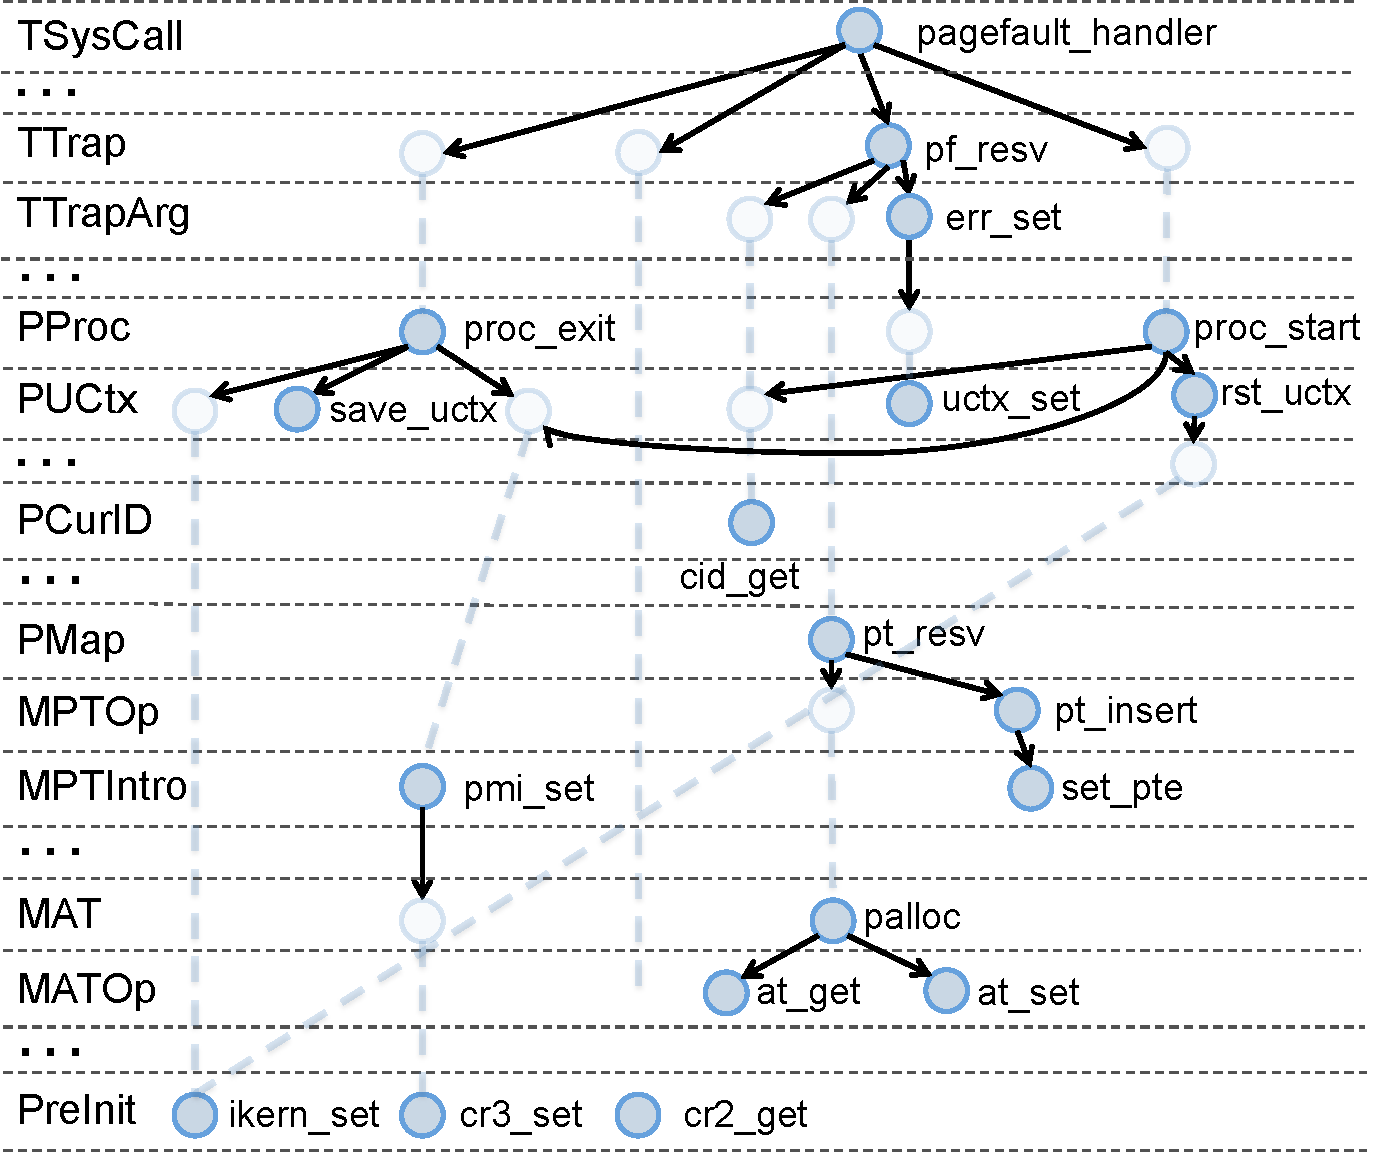
\includegraphics[scale=0.33]{figs/pagefault2}	
\caption{Call graph of page fault handler}
\label{fig:base:pagefault}
\end{center}
\vspace*{-14pt}
\end{figure}
}
specifies the behaviors of exception handlers
(\eg, page fault handler), interrupt handlers (\eg, serial port),
and system calls (\eg. IPC). It also specifies the behavior of ring switch and saving/restoring trap frames.
}
\ignore{
For example, a page fault at the user level traps into the kernel, saves the
current trap frame (done by both the hardware and software), and then jumps
to the page fault handler.
The page fault handler reserves a page for \texttt{PFLA} (if necessary)
and returns to the user level by restoring the saved user context.
The verification of the page fault handler depends on objects
introduced at various abstraction levels. 
\ronghui{So what? Everybody knows what is a page fault?}
% (see Fig.~\ref{fig:base:pagefault}).
}

\ignore{
Therefore, the behavior of the page fault handler is interpreted by
the concrete first-class code pointer until all the dependent layer
objects are introduced.  Then the handler code is verified and
the behavior is interpreted using its abstract atomic specification.
}

\subsection{Verification of user code}
To further simplify the reasoning about user code, we have implemented and
verified the user level system call libraries directly in the user space.
Since our machine semantics models hardware behaviors
like paging and ring switch, the specifications of user system call
libraries closely correspond to the real execution model in the actual
hardware. With this \emph{atomic} system call semantics in the user level,
the user code can be proved much more easily.

The top layer of \mCTOSbase{} offers a set of system calls for user programs, 
such as IPC calls and calls to trigger the scheduler.
The specifications of system calls are defined and verified at the user level
by wrapping the system call handler's specification
with the ring switch specification.
We can reason about user-level programs directly with these atomic system calls' specifications.


\ignore{
\newman{Already in Section 2}
\subsection{Other properties}
Except for the above features, we also prove the following properties of \mCTOSbase{}:
\begin{itemize}
\item Since the contextual refinement is termination sensitive, we prove the total
correctness of our kernel, meaning that our kernel will not get stuck
and all system calls for user program will terminate.
\item There is no integer overflow inside the kernel.
\item There is not stack overflow inside the kernel. (Statically checked by the analysis tool,
refer to Quentin's work)
\item All the pointers stored in the kernel objects are valid.
\end{itemize}
}
